\documentclass{wx672ctexart}

\usepackage{wx672bib}
\addbibresource{bib/os.bib}
\usepackage{wx672hyperref,wx672tikz}
\usepackage{amsmath,amsfonts,amssymb}

\usepackage{graphicx}

\usepackage[includemp,top=2cm,bottom=2cm,left=1cm,right=5mm,marginparwidth=8cm]{geometry}

\usepackage{enumitem}
\setlist{nosep}

\usepackage[toc]{multitoc}
\renewcommand*{\multicolumntoc}{2}
\setlength{\columnseprule}{.1pt}

\usepackage{wx672minted}
\usepackage{capt-of}% \captionof

\pagestyle{plain}

%\setcounter{tocdepth}{3}

% \newcommand\mpic[2][0pt]{%
%   \marginpar{\vskip#1\includegraphics[width=\marginparwidth]{thumbnails/#2}}}
\newcommand\mpic[1]{%
  \marginpar{\includegraphics[width=\marginparwidth]{thumbnails/#1}}}

\newcommand\mfig[3][]{
  \marginpar{%
    \centering\includegraphics[width=#1\marginparwidth]{thumbnails/#2}
    \captionof{figure}{\label{fig:#2}#3}}}


\author{王晓林\\{\ttfamily wx672ster@gmail.com}}
\date{\today}
\title{《Linux操作系统原理与应用》课堂讲稿}
\hypersetup{
 pdfauthor={王晓林},
 pdftitle={《Linux操作系统原理与应用》课堂讲稿},
 pdfkeywords={OS, Linux},
 pdfsubject={Operating Systems},
 pdfcreator={XeLaTeX}, 
 pdflang={Cn}}

\begin{document}

\newgeometry{left=3cm,right=3cm,bottom=2cm}
\maketitle
\tableofcontents

\begin{itemize}
\item 幻灯片:\url{https://cs6.swfu.edu.cn/~wx672/lecture_notes/os/slides/os-b.pdf}
\item 打印版:\url{https://cs6.swfu.edu.cn/~wx672/lecture_notes/os/slides/os-a.pdf}
\item 教材:\url{https://cs6.swfu.edu.cn/~wx672/lecture_notes/os/ref.html}
\item 实验:\url{https://cs6.swfu.edu.cn/~wx672/lecture_notes/os/lab.html}
\item 代码:\url{https://cs6.swfu.edu.cn/~wx672/lecture_notes/os/src/}
\item Debian安装指导:\url{https://cs6.swfu.edu.cn/~wx672/debian-install/install.html}
\end{itemize}

\printbibliography[title={参考书目}]

\clearpage
\section{老生常谈}
\label{sec:orgaeba803}

我提供的讲义、幻灯片、参考书等所有资料都是英文的,这有几方面原因。首先,英文真的很重要。怎
么算是重要?我们来举个例子,假设我现在给你留一个作业,比如写一个简单的system call吧。面对
这个作业,你会发现有诸多困难要克服:
\begin{enumerate}
\item 不知道什么是system call;(缺乏操作系统的相关知识)
\item C编程啊?不会;
\item 你说的这个编辑器(Emacs, Vim)我也没用过;
\item 没标准答案?要我上网搜什么?
\item 你提供的参考资料都是英文的?
\item 这作业太难了……(我没这份耐心)
\end{enumerate}

也就是说,想完成作业的话,你要克服上面这6个困难才行。而且,上面这6条,是我按它们的重要程度
排好了顺序的。其中最重要的是“耐心”,最不重要的是“操作系统知识”。为什么?因为,你们敷衍完这
门课之后,恐怕没有谁会去搞操作系统开发。可是,无论你将来做什么,只要你想稍微做出点样子,你
都必须要有“耐心”。
\begin{enumerate}
\item 耐心,无论干什么,都需要;
\item 英文,只要想找个好工作,就需要;
\item 上网搜,也就是科研能力,如果你将来搞技术工作,那么肯定需要;
\item 编辑器,也就是软件工具,只要你用电脑就需要;
\item 编程,只有程序员才需要;
\item 操作系统,只有搞系统开发才需要。
\end{enumerate}

也就是说,最通用的才最有用。尽管你以后不搞系统开发,甚至都不搞技术,但既然选了这门课,总该
有点收获,那就借着这门课的机会,补习一下你的英文吧。如果你打算将来吃技术饭,那么英文就更加
重要了。现代IT技术,都是西方人搞出来的,低头看看键盘,上面就没有一个中国字,不老老实实把英
文学好,你的专业技术也不会有什么前途。

面对这份作业,我相信大家完成作业的速度和质量也会大不一样。通常,好同学会完成得又快又好,为
什么?因为学习有“捷径”呗。好同学的捷径是什么?是这样:
\begin{enumerate}
\item 他做事的耐心早就锻炼出来了;
\item 他的英文已经学得不错了;
\item 他经常Google英文资料,而不是百度中文资料(上世纪90年代,中国人发出的第一封email,内
容就是「跨越长城,走向世界」。你指望靠坐井观天来振兴中华吗?);
\item 他Linux用得很熟;
\item 他C编程也不错;
\item 他唯一需要现学的就是一点操作系统知识。
\end{enumerate}

也就是说,貌似你们是同时开始做作业,同时开始克服这6个困难,但实际上,他已经提前把5个困难克
服掉了,而你是从现在才开始启动,所以他当然比你做得快、做得好。所谓捷径,无非是笨鸟先飞罢了。

「也不全是吧,老师,那孩子真的比我聪明」。聪明不重要,至少在本科学习阶段,真的不重要。这不
是说聪明不好,就好比电脑的CPU,当然是越快越好。但只是硬件好,软件很烂,电脑也做不出什么正
经事。如果你真感觉聪明不足,那么可以学点不需要聪明的东西,比如英文。英国的傻子都比我们英
文好,不是吗?可你的英文为什么这么烂?很简单,因为你懒。

「英国的傻子有良好的“语境”」。那么,你的高中同学英语都和你一样烂吗?和你同龄的年轻人,他们
考进了清华、北大、云大……英语显然比你强。所以,别扯什么“语境”的淡了,懒就是懒。发现问题,正
视问题,才可能解决问题。真想学好,就好好学。学习是需要耐心的,像长跑一样,只有气喘吁吁、
大汗淋漓,才算是锻炼,才能锻炼出强健的体魄。

\subsection{关于作业}
\label{sec:orgd04aec4}

下周一,我应该可以收到你们的作业了吧?「还什么都没讲,怎么做作业啊?」因为我布置的作业很简
单,就是每周问一个问题而已。因为我还什么都没讲,你还什么都没学,所以你满脑子都应该是问题,
问一个出来有什么难的?话虽如此,但提问有提问的规矩,要有条有理。
\begin{enumerate}
\item 我要做一件什么事情?
\item 我是怎样做的?(也就是步骤)
\item 做到哪一步的时候,我期待看到怎样的结果,可实际上看到的却是……
\item 于是我尝试了如此种种若干办法去解决它;
\item 我在这个问题上花费了多少小时?
\end{enumerate}

很显然,这个作业的意义就在于“做事情”。如果你能保证每周做一件稍微像样的事情,花费若干小时真
正去克服一些困难,那么你在毕业的时候就可以傲视身边这群懒蛋了。“傲视懒蛋”,这真的算不上有出
息,但这至少是第一步。想有出息,就要时刻提醒自己「我未来的竞争对手绝不是身边这些比我更懒的
游戏帅哥、追剧美眉」。想有出息,就要去和校外比,和省外比,和国外比。

「可是,我真的想不到有什么正经事要做啊」。如果你打算有出息,只是对操作系统缺乏兴趣,那么没
关系,我说过了,操作系统是学习中最不重要的事情。你尽管去做你感兴趣的事情,然后在作业里告诉
我,你是怎样做的,花了多少小时,克服了哪些困难?更直白地说,只要你给我一个好印象,期末考试
是不成问题的。

「我还是不知道该做啥,你分配个任务让我做吧」。千万不要找我要任务,因为我对「这是老师让我写
的,那是家长逼我学的」深恶痛绝。为什么?因为这些都是“借口”,是为失败找的借口,是为敷衍了事、
推卸责任找的借口。扯淡的是,从幼儿园到大学,我们的教育一直在为你提供这些借口。换言之,我们
的教育一直在培养“敷衍了事、推卸责任、毫无担当”的人。只有“尊重个人权利、尊重个人自由”的教育
才能培养出“负责任、有胆当”的人。显然,全世界没有哪个国家100\%实现了这种理想化教育。但我们也
看到,欧美国家的孩子动手能力更强,更有团队精神。为什么?因为这些孩子从小就被鼓励去做他们自
己喜欢做的事情。既然是自己的事情,自然会认真去做。「我要做什么,我该怎样做」这样的问题对他
们来讲,是家常便饭。久而久之,就养成了认真、负责的做事习惯。

我一个人没本事改变教育现状,但至少在我的课堂上,我们可以尝试一下。现在我给你机会,自由自在
地去做自己想做的事情。我希望你珍惜它。

\restoregeometry
\section{概述}
\subsection{什么是操作系统?}
\label{sec:org22d570f}

我们还是按着幻灯片的顺序来上课吧。其实,大家心里都明白,上课和学习是两码事,就好像“做一天
和尚”和“撞一天钟”是两码事一样。来课堂不等于就学习,学习也未必非要上课。毕竟,在课堂上我能
告诉你的充其量就是「你该学些什么」,而真正的学习肯定是课下进行的。“修行”不是“撞钟”能取代的。

好了,我们现在步入正题。前面说了,正题(也就是操作系统知识)并不重要,如果你真要学习的话,
千万不要绕过前面五个困难,直奔第六个,也就是最不重要的操作系统。你应该静下心来,克服幻灯片
里的每一个生词,认真理解这张幻灯片要表达的意思,这需要你去查阅参考书里的相关章节。然后,在
你认为「我终于搞明白了」的时候,把书合上,把幻灯片关掉,然后用自己的话把幻灯片里的内容复述
出来。没错,这才叫“学习”。

好了,假装你还没被吓跑,我开始讲第7张幻灯片,What's an OS?\mpic{pg_0007}
第一句说,OS就是当你网购一个OS
的时候,人家寄给你的东西,那肯定就是OS。没错,这话很正确啊,虽然只是个玩笑,但并非毫无意义。
起码这句话让我意识到,要和流氓正经讲道理该有多困难。人家只要回你一句这么“正确”的话,就能噎得
你想撞墙。人嘴两张皮,人嘴是多么邪恶的两张皮啊!所以说,道理永远是讲给“讲道理的人”听的。对
于不讲道理的人呢?用他听得懂的语言去教训他!说白了,给他不及格呗。

好了,再看第二句,OS是从一开机就开始跑,直到关机(或者死机,如果你用Windows的话)才会结束
的程序。这句话算是很讲道理了。这的确是OS的重要特征之一,可以算是操作系统定义的一部分了。

第三句,它是资源的管理者。那么,什么是资源?电脑诞生之前,资源这个词就存在了。水、土地、煤
炭、石油、空气、人、动物……貌似没有什么东西不能被当作资源。没错,就连“垃圾”也可以被认为是
“放错了地方的资源”。但通常,当我们谈到资源的时候,“空气”和“垃圾”都不太容易被想到,为什么?
因为它们不“紧缺”。当我们谈资源的时候,通常是在谈那些“大家都想抢的东西”。

回到电脑里面来,也一样,everything is a resource,但大家(众多进程)无时无刻不想抢的东西就
两样,一是time,时间;二是space,空间。和时间相关的资源就是CPU,和空间相关的就是内存。好了,
现在打开终端,跟我学一个小命令:

\begin{minted}[mathescape=true,linenos=true,numbersep=5pt,frame=lines,framesep=2mm]{sh}
ps aux | wc -l
\end{minted}

用这条命令可以数出你的电脑里正运行着多少个进程。我的是191个。而我的CPU是8核,也就是说,191
个进程要抢着用8个CPU,没人管肯定是不行的吧。任何一个程序要运行的话,先要把它加载到内存中去,
而我的内存只有8G,如果不够用怎么办呢?操作系统最重要的工作就是负责CPU和内存的分配与管理,
它是电脑里的resource manager。

第四句,它是个控制程序。假如那191个进程里,谁和谁发生了不愉快,比如一个流氓进程非要往我的
地址空间里写东西,那么,操作系统肯定要出手干预,或者在流氓得手之后,帮它洗地。每当此时,你
心爱的Windows就会呈现出著名的Blue screen of death。Unix没这么夸张,它通常会在你启动流
氓程序的瞬间,就告诉你“Segmentation fault”,也就是所谓“段错误”,这通常是访问非法内存地址造
成的。

最后一句,关于操作系统,并不存在一个放之四海而皆准的定义。为什么呢?因为有个问题,操作系统除
了要一直转着不停,除了要管理资源,除了要洗地之外,还应该有那些功能呢?这就见仁见智了。举例
而言吧,苹果和微软都把图形界面放到了操作系统内核里,因为这样“打开窗户的速度”更快;而其它的
Unix,还有Linux,内核里都不包含图形界面,因为并不是所有人都需要图形界面,比如服务器就不需
要图形界面。庞大的图形界面会给内核带来更多的bug,降低系统的稳定性、安全性、和效率。因此,
专业的服务器都不太会选用Windows或者苹果系统,毕竟Windows和苹果的设计初衷,就是面向个人电脑
用户。服务器的话,基本上都是Linux和Unix的天下(除了苹果,虽然它也算是Unix)。Linux、
Windows、苹果,这些都是通用型操作系统,这世界上还有很多专用型系统呢,比如用于流水线控制的
单板机。不同的系统,面向不同的工作场景,有不同的设计需求,所以,操作系统该如何定义呢?还是
见仁见智吧。

好了,现在关掉幻灯片,把你的理解复述出来吧,最好用英文。

\subsection{OS的功能模块}
\label{sec:org8c45b76}
\mpic{pg_0008}幻灯片第8页上这张图,简化一下,就是图\ref{fig:os}所示的样子。
\mfig{os}{OS}
左、右两张图是一回事,表达的是同一个意思,我们,生物意义上的人,从来不直接使用操作系统,我
们只使用应用程序,应用程序才会去和操作系统打交道。任何应用程序如果想使用硬件(比如键盘、鼠
标、显示器)的话,都要向操作系统发出请求,然后操作系统帮你把键盘输入的字符显示到屏幕上。

「干吗这么费事?没有操作系统不行吗?」,其实前面我们已经回答过这个问题了,电脑里的资源(比
如键盘、鼠标、显示器)很紧缺,若干进程都要抢着用,所以必然需要有人来维持一下秩序。换言之,
如果你的系统里只跑一个程序的话,也就是所谓“单任务系统”,那么操作系统的确就显得多余了。

把上图中的OS放到显微镜下,看到的就是第8页的幻灯片。片中上下两条虚线之间就是我们最关心的部
分,操作系统。它是个软件,可以很庞大而复杂,也可以小巧而简单,因设计需求的不同而变化。通常,
讲课的时候,都选庞大而复杂的来说,而具体编程实现的时候,都是怎么简单怎么来。为什么?因为说
起来容易,做起来难呗。

无论如何,一个通常意义的操作系统,它里面会有进程控制、内存管理、文件系统、输入输出等功能模
块。教科书上,一般也是着重讲这几个模块。我们16周的课,通常只能讲完前三个,输入输出就靠自学
了。本来嘛,上课也就能告诉你“该学什么”,不是吗?

现在来看看,APPs是如何向OS请求服务的?APPs和OS都是软件,软件之间怎么相互通信,或者说传递数
据啊?函数调用呗。所以说,APPs只要调用OS提供的函数,就可以把信息发送给OS了。每个操作系统都
为用户进程提供了一整套函数,或者说一个“函数库”,这个函数库就是图中的system call interface。
Linux的库比较小,里面有大约400个syscall。Meanwhile,Windows的库里有4000多个。是大点好,还
是小点好呢?其实很好回答,就问问你自己,「做为一个程序员,我是愿意看一本400页的手册呢,还
是看4000页的?」。分手吧,她真的太胖了!而且,不止是手册的厚薄问题,软件的代码量越大,
bug数量必然就越多。这可是操作系统啊,它蓝屏,我一点都不觉得意外。

再注意一下,图中的syscall interface有两条路通往用户程序。一条路是直接的;另一条是间接的,
要通过libraries(函数库)。其实,这个函数库,差不多就是专指C函数库。它不在OS里面,它在用户
层(user level),是一个普通用户就能随意安装、卸载、替换的软件包。既然有一条直接的路径,为
什么还需要它?有两个主要原因:
\begin{enumerate}
\item 跨平台。前面说了,不同的OS提供了不同的syscall函数库。那么,如果你在windows平台写了个程
序,里面自然要用到Windows提供的syscall,比如说 \texttt{CreateProcess()} ,用来产生一个子进程。
写好了之后,你编译、运行,一切良好。于是,你把它拿到Linux平台,直接运行肯定是不行的。换
了平台,要先编译。「完蛋了!在Windows上一切都好好的,为什么到Linux上就编译通不过?Linux
太难用了!」没错,Linux对你不友好,也只是对“你”不友好。为什么?因为(此处略去500脏字)。

想想看,Windows提供了4000多个syscall,其中包括 \texttt{CreateProcess()}; 而Linux只提供了400个,
你保证它也有 \texttt{CreateProcess()} 吗?Too simple, sometimes naive!在Linux平台,想要产生子
进程的话,你要调用 \texttt{fork(2)}. 于是,累了,你不得不把程序中用到的成百上千个Windows
syscall都替换成相应的Linux syscall!我相信你的脏字也会很多的。结论,由于你直接调用了
OS提供的syscall,导致你的软件可移植性极差,根本不跨平台。

如果你不直接调用syscall,而是“走弯路”,调用Library里的函数,生活就美好多了。比如说,我
们最常用的Library是POSIX提供的LIBC,它既有Windows版,也有Linux版。于是,你只要在Windows
和Linux上都装好POSIX LIBC,编程的时候调用里面的函数,让它去帮你调用底层的syscall,就没
问题了。
\item 方便。函数库存在的意义,不止是把syscall包装一下,以便于你的软件可以跨平台。它还提供了很
多广受用户欢迎,而syscall没有提供的功能。比如说 \texttt{printf(3)} 吧,
\begin{minted}[mathescape=true,linenos=true,numbersep=5pt,frame=lines,framesep=2mm]{c}
printf("Hello, world!\n");
\end{minted}
说简单了,它的功能就是“屏幕输出”。但直接调用syscall(不考虑跨平台的话) \texttt{write(2)} 也可
以实现屏幕输出。实际上, \texttt{printf(3)} 最终就是通过调用 \texttt{write(2)} 来完成屏幕输出的。
\begin{minted}[mathescape=true,linenos=true,numbersep=5pt,frame=lines,framesep=2mm]{c}
write(1, "Hello, world!\n", 14);
\end{minted}

这么绕弯的好处是什么呢? \texttt{printf(3)} 提供了带格式的输出,而 \texttt{write(2)} 不行。为什么
\texttt{write(2)} 不提供格式支持呢?原因既浅显又重要,Linux的设计者认为,OS只应该提供“不得不提供
的功能”,所有非必须的功能都应该由用户层软件提供。这也是Linux内核不提供GUI(图形界面)支
持的原因。这也是它更适合用来做服务器的原因。

「圆括号里的 \texttt{2, 3} 是什么意思?」 \texttt{2} 代表syscall; \texttt{3} 代表libcall。
\end{enumerate}

再来看看图中的这两条路,边上都有一个单词,trap,当名词用的时候被翻译成“陷阱”。但是,在计算
机专业,它经常被用做动词,是“触发”的意思。一个陷阱挖好了,只要别踩它,什么事都没有。一旦你
踩上去,就会触发你的噩梦……同样,用户程序以调用函数的方式触发操作系统的某个功能,所以这里用
trap一词。

后面的课程里,我们还会经常接触system call。课上用到的例子,自己去尝试一下吧。
\begin{itemize}
\item \url{https://cs6.swfu.edu.cn/\~wx672/lecture\_notes/os/src.tgz}
\item \url{https://cs6.swfu.edu.cn/\~wx672/lecture\_notes/linux-app/src.tgz}
\end{itemize}

\subsection{选个OS}
\label{sec:org50cf3aa}

\mpic{pg_0009}这张画在技术圈里还是挺著名的,而且有好几个版本。不论哪个版本,都是个笑话。能
看懂的,就笑呗;看不懂的呢,“加油!不哭!”,画一个自己的版本,咱们再笑呗。

「我是学技术的,到底该用哪个系统啊?」。肯定不该用Windows。为什么?
\begin{enumerate}
\item 学外科的,总得解剖过尸体吧;学操作系统的,总得解剖过操作系统吧。Windows根本就不开源,你
看不到它里面的东西,所以无法拿它来解剖、学习。如果你真的有本事把它解剖了,那么你就要收
到法院的传票了,因为这犯法。
\item Windows是要花钱买的,不便宜,而且在它的版权声明里还罗列着种种限制,包括不能修改、不能送
人、不能私自买卖……而Linux是自由软件,你可以自由获取、自由使用、自由学习、自由送人、自由
买卖、自由修改…… 你一个穷学生,不该为爹妈省点钱吗?而且,这绝不只是钱的事情,「自由」才
是最重要的。武汉的李文亮大夫用生命告诉我们「言论自由关系到每个人的生命安全」。西谚有云
「Live free or die」,先贤译之为「不自由,毋宁死」。看看李大夫,我的翻译是「不自由,真
要命」。
\item 「可是我身边的同学和老师,他们都用Windows啊」。没错,而且我劝过他们了,就像我劝你一样。
他们会说「自由了,早晚不也得死」,「不觉不自由,也就自由了」,「现在不挺舒服的,自由又
不能当饭吃」,「干吗非得跟人不一样啊」……的确,各有各的活法,至少我也要尊重他们「选择不
自由」的自由。而且,被这些人环绕着,你会感觉自己才是个怪物。又想起一句西谚「Birds born
in a cage think flying is an illness」,笼子里长大的鸟会认为飞翔是一种病。你的翅膀还在
吗?愿意做一个飞翔的“怪物”吗?还是收起翅膀,和他们一起做“正常人”呢?西洋人又说了,「Why
fit in, when you were born to stand out?」,一个生来就该与众不同、卓尔不群的人,干吗又
要去随大流呢?
\item 用Linux的同学,毕业后的前景都很好。这并不意外吧。首先,肯用Linux的同学都普遍比较好学;
其次,用Windows的人太多,竞争自然就大。竞争大,老板就会把工资压得很低。而用Linux的人少,
所以需求缺口巨大,工作自然要容易找,工资也相对较高。
\end{enumerate}

好了,晓之以理、动之以情、诱之以利,我都做到了。关于什么是GNU/Linux,很久以前我翻译过一篇
《Linux简史》,大家可以看看。
\begin{itemize}
\item \url{https://cs6.swfu.edu.cn/\~wx672/lecture\_notes/linux/linux\_history/}
\end{itemize}

「好吧,我可以试试,那我到底该装哪款Linux呢?」。
很简单,你周围的人用哪个,你就用哪个。为什么?容易得到帮助呗。所以,最好是我用哪个,你就用
哪个。跟着我的安装指导一步步走,应该不会很费事。
\begin{itemize}
\item \url{https://cs6.swfu.edu.cn/\~wx672/debian-install/install.html}
\end{itemize}

\subsection{抽象}
\label{sec:orgc6f1cc9}\mpic{pg_0010}
Abstraction,抽象,就是把不想看到的细节都藏起来。为啥藏起来?因为懒呗。尽管“the devil is
in the detail”,但多一事不如少一事,什么都看那么清楚,还怎么岁月静好啊?其实,抽象不止是
“需求”,而且是我们的本能。在和岁静美女谈诗和远方的时候,你肯定不愿意被她肠子里的细节打扰,
因为那是肛肠科大夫的事情。

同样,计算机系统也是五脏俱全,为了避免被细节困扰,工程师们发明了一大堆抽象概念。比如,
文件、虚拟内存、指令集、进程、虚拟机,等等。

先说说文件。电脑里的文件是我们虚构出来的东西,是个概念。电脑是用来处理数据的,而数据存储在
硬盘(或者其它什么盘)上。如果你没拆过硬盘的话,可以……算了,赚钱不易,还是别拆了,看看解剖
图就好。比如下面这个:
\begin{itemize}
\item \url{https://www.aresgroupofcompanies.com/hard-disk-structure/}
\end{itemize}

硬盘里用来记录数据的东西就是一摞圆形金属片(platter)。这个薄薄的platter很像光盘,上面有一
圈圈的细纹路,叫磁道(track)。把这些小薄片摞起来,就形成了一个圆柱。现在,你可以把这个圆
柱想象成一个树桩,截面上布满了年轮(就是圆片上的track嘛)。实际上一圈圈的年轮就对应着一个
个粗细不同的圆柱。我们把这一圈圈的圆柱叫做柱面(cylinder)。数据就存放在这些cylinder上。那
么,想要读取数据的话,你得告诉我,你要读取哪块硬盘上的哪个柱面上的哪个磁道上的哪一段(扇区,
sector)数据。用程序员的方式来表达就是写个函数呗:
\begin{minted}[mathescape=true,linenos=true,numbersep=5pt,frame=lines,framesep=2mm]{c}
read(drive, cylinder, track, sector)
\end{minted}
这函数名字叫 \texttt{read} ,它携带4个参数,分别是硬盘号、柱面号、磁道号、和扇区号。而且这函数只
能用来读硬盘,如果是光盘、U盘、软盘呢?这么多琐碎的细节都要考虑啊,还让不让人岁月静好了!
在烦死了若干工程师之后,全世界讨厌细节的工程师们联合了起来,他们发明了“文件”这个概念。其实
算不上发明,因为在电脑存在之前,文件就已经存在了,我们不过是借用而已。无论如何,自从有了
“文件”的概念,岁月就静好了。现在读取数据,只要:

\begin{minted}[mathescape=true,linenos=true,numbersep=5pt,frame=lines,framesep=2mm]{c}
read(filename)
\end{minted}

也就是说,在读数据的时候,我们只需要提供文件的名字就可以了,甚至不需要操心读的是硬
盘、软盘、光盘、U盘、还是网卡。感慨一下,这世界上哪里有什么岁月静好,无非是有人替你寻衅滋
事罢了。再回来看看幻灯片,files是对什么的抽象?I/O devices。所有这些盘,和声卡、网卡、显卡、
键盘、鼠标……都是I/O设备。没错,in Unix, everything is a file.

再来看看虚拟内存,它是对主内存和文件的抽象。虚拟内存的概念当然不会就这么简单,后面我们讲内
存管理的时候,会着重来探讨。现在嘛,你至少该意识到,内存绝不只是主板上那个内存条,文件(这
盘、那盘、这卡、那卡)都可能被用做内存。这么多琐碎的细节是需要创造个新概念来代表一下的。

同样,汇编指令集被用来代表CPU的具体结构;进程被用来代表系统运行的复杂状态;虚拟机被用来代
表我说不明白、你听不懂的所有东西。
\subsection{设计目标}
\label{sec:org587643a}
\mpic{pg_0011}
任何系统的设计都要考虑到这两件事情,一是方便;二是效率。任何系统都是这两个因素权衡与折衷的
产物。所谓“方便”,当然是为人(操作者)考虑的。“以人为本”的典范,除了伟大的党,就要数苹果了。
Windows的界面也很友好,但它是抄袭人家苹果的,当年两家还为此打了多年的官司,后来私了了。

“方便”不是没有代价的,它要耗费可观的系统资源。所有图形界面(GUI)都很庞大,耗硬盘、耗内存、
耗CPU。所以,在硬盘、内存、CPU都很寒酸的“古代”,系统设计是绝对不会考虑这些东西的。古老的
Unix,它提供给用户的界面是终端(terminal)。所谓terminal,就是一个键盘和一个打印机。当年连
显示屏幕都没有,从键盘输入个命令,回车之后,运行结果直接打印到纸上。

「可那是古代啊,现在干吗还要使用终端命令行呢?」。这问题很值得我们思考。先回答我的问题吧,
「学习到底该学些什么?」刚问出这个问题,我又想到了另一个问题,「学习的目的是什么?」在我看,
学习不是为了获得知识,至少首要目标不是。为什么呢?你想啊,大学里要学上百门课程,最终在工作
中能用到的有多少?去问问那些毕了业的师哥师姐,他们会告诉你,能用到的课堂知识不超过5\%。所以,
学习如果是为了获得知识,把剩下那95\%扔到也没啥不可以;学习如果是为了获得答案,考试的时候,
把头偏得远一点就看见了。

学习不是为了知识和答案,而是获得知识和答案的过程,是在书山学海中挣扎,气喘吁吁,大汗淋漓,
枯燥乏味,马拉松长跑一样的过程。通过这个痛苦的过程,你能获得强大的学习能力。有了能力,在工
作中遇到的任何新挑战,你都可以快速学习,快速上手。所以,如果你放弃了那95\%的课程,那么你就
放弃了95\%的训练机会。没有训练,哪有能力?由此再进一步,你应该意识到所谓“一招鲜,吃遍天”实
在是文凭贩子们的“害人的偏方”,因为它让你心安理得地放弃了几乎所有的训练机会。

好了,说回来,那5\%能被用到的是什么?其实就是最通用的东西,算数、语文、英语。「除此之外,总
要学点技术吧」,那就学点“经典的”东西。什么算是经典?终端命令行就是。从1969年开始,一直被用
到现在,系统管理员离了它就活不下去,这就是经典。为什么非要用命令行?
\begin{enumerate}
\item 服务器不欢迎图形界面,因为bug多,而且耗资源。既然没有GUI,那么鼠标自然也就用不上了。
\item 服务器大多是远程维护的,因为它辐射大(CPU多)、噪音大(风扇多),没人愿意在服务器边上工
作。既然是远程,当然要联网。举个例子,如果我想看看远端服务器里有哪些文件,只要敲命令 \texttt{ls}
再回车就行了。也就是说只要通过网线把3个字节的数据(l, s, 回车)发送过去。而如果是利用图
形化的远程桌面呢?要从远端服务器传送一个窗户过来,然后你每敲一次鼠标,窗户还要刷新一次。
一个窗户的图像有多少字节?3K不止吧。也就是说,远程桌面所耗费的网络带宽是命令行的一千倍
以上。你觉得哪个效率高呢?如果网络不通畅呢?
\item 从学习的角度来说,我们很多同学,不夸张地说,临毕业了都不太会用键盘。计科专业的学生啊,
好意思吗?又可以发挥一下想象力了,一个班都在敲鼠标的时候,只有你是在用键盘做事情。我觉
得,找到女朋友的概率也会高不少吧。学习就是摆脱坏习惯,养成好习惯的过程。不妨就从摆脱鼠
标依赖开始吧。
\end{enumerate}

\subsection{OS简史}
\label{sec:org0af235d}

看看幻灯片第12页上这张画\mpic{pg_0012}\citetitle[Sec.~1.2.2]{tanenbaum2015modern},左边的帅
哥明显是个程序员,手里拿着他的程序。古代没有硬盘,程序都是记录在长长的纸带上,像一大卷卫生
纸。纸上打孔的地方代表0,没打孔就代表1,于是长纸带上就密密麻麻地布满了程序。为了能运行程序,
他要把纸带拿到机房来,放到Card reader里面,然后纸带上的程序就被读了出来,并被写到磁带上
(Tape drive就是磁带机)。美女显然是看机房的,她取过磁带,放到中间主机的磁带机里,然后开动
主机。主机从Input tape读取程序,进行运算,再把输出结果写到Output tape上。最后,打印出来,交
给帅哥。

古代的电脑就是这样工作的。那么,请告诉我,操作系统在哪儿?其实很简单,想想谁是Resource
manager?谁在控制程序?很显然,是美女!如果有若干帅哥排队的话,她决定先运行谁的程序。如果
出现了卡带之类的问题的话,她负责洗地。也就是说,当年的计算机都是“单任务系统”,根本不需要操
作系统。后来,硬件越来越强大,“单任务”就显得很浪费了。为了应付“多任务”的新局面,才逐渐演变
出了操作系统。

最早的现代意义上的操作系统诞生于1969年。那年夏天,当Neil Armstrong在月球上迈出那“一小步”的
时候,贝尔实验室里以Ken Thompson和Dennis Ritchie为首的几个年轻人用B语言和汇编语言,花4周时
间实现了一个现代操作系统的雏形。之后,为了提高系统性能,他们决定放弃B语言。于是Ritchie说,
「那我写个新的语言吧」,Let there be C!于是,就有了C。没错,C语言是为Unix而诞生的。那么,
我们学C编程该用什么系统呢?Linux已经存在二十余年了,它自由、开源、免费、优秀,而我们的编程
课还在用不自由、不开源、不免费、染病毒、常蓝屏的Windows,这个国家病了,但病的绝不止是武汉!
1973年,用C重写的Unix系统诞生了。那四千余行代码,到今天还是程序员心中的圣物,因为它就是软
件世界的“Let there be light”。

从Unix到Linux中间还有很多有趣的故事,有空再聊吧。或者看看我翻译
的\href{https://cs6.swfu.edu.cn/\~wx672/lecture\_notes/linux/linux\_history/}{《Linux简
  史》}。

\label{sec:org1ad1b10}
幻灯片第13页\mpic{pg_0013}上展示的是硬件的进化历程。第一代计算机是电子管做的。中国人在看上
电视之前,家里一般都会有个“广播匣子”,也就是电子管收音机。我家那台是上海产的美多牌。那时候
的小孩儿趁家长不在家的时候,肯定都拆过它的后盖,一窥究竟。在这个两尺长、一尺宽、一尺多高的
长方盒子里,平放着一块薄木板(plug board),上面插着一些手指头大小的真空玻璃管(vacuum
tube),管里有一些银光闪闪的金属丝、金属片。伸出两个管脚的就是二极管,伸出三个的就是三极管。
通上电的时候,会微微发出红光,像个灯泡。如果哪天收音机不响了,那么拆下后盖,肯定会发现某个
电子管变黑了,就类似烧坏了的灯泡。把它拔下来,换上个新的就行了。小孩子手欠,总喜欢玩匣子上
的音量、调频旋钮。如果不小心扭到了短波上,家长肯定会飞奔过来打手,因为偷听敌台是要坐牢的。
现在满脑子都在唱罗大佑的《童年》……  电子管的计算机,中国人都没见过,估计也和收音机差不太多
吧。没有小说连续广播,没啥好玩的。

后来,科技发展了,有了晶体管(transistors),收音机也都升级成了晶体管的,只有巴掌大小,不
如电子管的气派。晶体管的计算机,咱也都没见过,书上说它已经可以批量地运行程序了,这就是所谓
“批处理系统”(batch system)。所谓“批处理”,就是把程序排好队,一个接一个地运行。

再后来,有了集成电路(IC,Integrated Circuit),也就是有了芯片(computer chip),也就是说,
计算机硬件发展到了现代。软件革命也随之而来,以Unix为代表的“多任务系统”诞生了。所谓“多任务
系统”,也就是传说中的“分时系统”(time-sharing system)。智计无双、武绝天下的丐帮帮主黄蓉,
强敌环伺之中,临危不乱,荧荧绿棒随手挥出,只一招“天下无狗”,那十余条大汉便都被点中了穴道。
再一招“拨狗朝天”,连环挑出,只一瞬间,众贼人便齐刷刷摔将出去。这就叫分时处理,太快,每个大
汉都感觉黄帮主是专虐他一个。十余个任务瞬间(近乎同时)就完成了。

再后来,电脑硬件在本质上没有更多的变化,只是越来越快,越来越小,越来越便宜。1980年,IBM说:
“Let there be PC”,个人电脑就“飞入寻常百姓家”了。每一台IBM PC机,以及随后出现的山寨PC机
(IBM兼容机),里面都装的是比尔·盖茨的MS-DOS系统。为什么不装Unix?当年,Unix主要面向大型机
(main frame),它的买主都是企业、大学、政府机关、科研机构。财大气粗的AT\&T根本没把玩具一样
的PC机放在眼里。比尔·盖茨比AT\&T有眼光(穷出来的),于是他发了大财。当然了,光有眼光也没戏,
每一个成功男人的背后都有一个不平凡的女人。盖茨的老妈是IBM的高管。

\subsection{多任务系统}
\label{sec:orged5e015}\mpic{pg_0014}
“多任务”(multi-tasking),也叫“多程序”(multi-programming),也叫“多进
程”(multi-processing)。以前,这几个词是有些分别的,但毕竟分别不大,所以后来就混着用了。
前面我们提到过,如果是“单任务”的话,操作系统有点多余。只有在“多任务”系统里,它才必须存在。
它的主要工作,包括
\begin{enumerate}
\item 工作调度。“调度”这个词比电脑要古老得多。在公交总站、机场、火车站,都有专门负责调度的部
门,从那里经常传出“你现在可以开车出发(或者起飞)了,其它车辆(或者飞机)等会儿”这样的
声音。调度的本质在于汽车公路、飞机跑道、火车铁轨这些“资源”的数量远小于汽车、飞机、火车
的数量。为了不打架,所以要调度。

所谓“工作调度”,job scheduling,它负责决定现在哪个程序应该被加载到内存中来。硬盘里有成
百上千的程序,任何一个程序要运行(也就是使用CPU)的话,必须被加载到内存中去。但内存一般
都比硬盘小很多很多很多,所以不可能把所有程序都加载进去。那么,该加载谁呢?由操作系统的
“工作调度”这个功能模块来决定。听起来很有道理,对吧?逗你玩儿呢。至少在我们的电脑上,根
本就没有“工作调度”这回事。很显然,你硬盘里有100个游戏、1000部电影,你现在要玩那个,看那
个,完全是由你自己决定的,是你自己用鼠标在那个“少儿不宜”上点了两下,把它加载到了内存里。

传说中,“工作调度”在批处理系统里比较常见。现在的批处理系统一般都用在超级计算机里。这些
super computer一般都用来做很庞大的运算,比如先花一星期模拟一下气候变化对地球的影响,
完事以后,再来模拟一下核冬天。都是传说,我也没见过。
\item 内存管理,memory management。任何一个程序,如果要运行它,都要先把它加载到内存中来。那么,
加载到内存中的什么地方呢?内存不够用怎么办呢?问题多着呢,后面我们再详细探讨。
\item CPU调度。我的电脑里(内存里)现在有近200个进程在运行着,但只有一个8核CPU。那么这个所谓
的“在运行着”就很假了,因为顶多能有8个进程在使用CPU,剩下的那些都只是在内存中呆着,等着
使用CPU而已。假如,现在有一个进程结束了,也就是说,有一个CPU空闲下来了,那么该把它交给
哪个“呆着”的进程呢?这就由“CPU调度”模块来决定。这个话题,后面我们也会专题讨论。
\item 进程管理,process management,这部分也很重要。怎样产生一个进程?子进程和父进程有什么牵
连?进程结束时该做些什么?进程之间怎样共享数据?怎样相互协调?这些问题,后面也会专题讨
论。
\end{enumerate}

\subsection{大大小小的OS}
\label{sec:org9696184}\mpic{pg_0015}

这一页就是告诉你,在不同的应用场合我们会见到不同的OS。Mainframe,就是所谓大型机。Frame是框
子、架子的意思。放在“主要大架子”里的机器自然就是大型机了,一个名符其实的庞然大物,比最大的
小汽车还要高大。运算能力嘛,在当年肯定算是很强。如此庞大、昂贵的设备,如果一次只给一个人用,
也就是大家排队用,那效率就太低了。所以,大型机里装的都是多用户、多任务系统,也就是Unix。
Unix的设计目标之一,就是要同时支持上千个用户。上千根线缆从主机箱伸出来,每根线缆的尽头连接
一个终端(terminal,键盘+打印机)。终端前,程序员正在聚精会神地玩游戏。没错,虽然当年的
Unix还很简陋,但Ken Thompson并没忘了为它开发一个游戏,Space Travel。

现在,随便一个手机的运算能力都比当年的大型机强,所以大型机就进了博物馆。取而代之的是超级计
算机,super computer,也就是用网线把很多普通的计算机连接起来,让它们共同完成某一个运算任务。
既然是很多普通机器,那么每个机器里肯定都要装操作系统喽?没错,而且为了方便管理,通常它们装
的都是同样的系统。2018年以后,全世界500强的超级计算机里,已经看不到其它系统了,都怪Linux。

再看看“实时系统”(real-time system)和“嵌入式系统(embedded system)”。所谓“实时”,是说系
统要能应付较苛刻的时间要求。比如说,用于生产汽车的流水线控制系统,一个汽车轱辘送到了面前,
机械手臂就要马上伸出去,拧上一个螺丝。而且,这个拧螺丝的动作必须要在一个很短的时间段内完成。
如果没能完成,那么,轱辘就过去了,于是,整个装配汽车的任务就失败了。再如,一个采样设备,
比如声纳吧,每一秒钟给你发送一次数据,那么你就要在一秒钟内完成接收处理。如果完不成,那么下
一秒的数据又到了,就更加来不及处理,只能丢弃掉。

实时系统通常都是专用系统,通常都很小巧,而且为了安全、可靠、快速,通常它们都是烧(或者说“刷”)
在ROM里面,而不是装在硬盘里。凡是刷在ROM里的系统,就叫“嵌入式系统”。比如,单板机系统就是典
型的嵌入式系统。以前,“实时”和“嵌入式”肯定是同时存在,所以总是被放在一起说,叫“实时嵌入式
系统”,或者“嵌入式实时系统”。现在,不好说了。比如,手机系统就是刷在ROM里,但Android一点也
不小巧,也不那么实时。

Smart card,就是我们说的智能卡,它上面也有系统吗?也许007用过吧,不管它。
\subsection{为人民服务}
\label{sec:orga0e95bc}\mpic{pg_0017}

在幻灯片的第10页,我们专门探讨过“抽象”是怎么回事。所谓“抽象”,就是把不想看见的细节藏起来。
“国家”和“计算机”一样,都是抽象概念。当我们说「用这台电脑发送一封email给女朋友」时,做为用
户,我们并不在意主板、CPU、内存、网卡、键盘、进程、文件……这些电脑里面的细节。同样,当我们
说「某个国家向太空发射了一颗卫星」时,我们也并不会想到山川、河流、煤矿、人民、文化……  这些
“国家”所涵盖的细节。如果说“为电脑服务”莫名其妙的话,那么“为国家服务”显然也不合逻辑。正确的
爱国姿势应该是“为人民服务”。

操作系统在电脑中的角色,完全等同于政府在国家中的角色,它就该是为人民服务的。毕竟人民公仆也
要吃饭嘛,所以政府自然要消耗掉一定的社会资源,但它显然不该消耗太多,不该吃得太胖。北朝鲜的
伟大公仆明显是吃得太饱了,所以老百姓就都面黄肌瘦。同理,做为软件,OS本身当然要消耗掉一定的
系统资源,但显然它不该消耗太多,它应该把尽量多的资源用于为用户进程服务。在这方面,Linux明
显比Windows要“清廉、高效”。

无论如何,操作系统的工作分为两大部分,一是服务人民,二是自我维护。本页幻灯片上列出了主要的
几点。关于服务人民:
\begin{enumerate}
\item 提供用户接口。注意,这个接口既不是你们的GUI(Graphical User Interface),也不是我的CLI
(Command Line Interface),而是System Calls,也就是OS与用户进程之间的接口。
\item 帮助程序运行(Program execution)。比如,把程序加载入内存,还要给它CPU用。也就是给进程
分配资源。
\item 输入/输出操作。输入/输出都要涉及到硬件,资源有限,不能想用就用,当然要OS来帮忙管理、调
度。
\item 文件系统操作。前文说过了,“文件”是OS为用户进程提供的抽象概念。用户对文件的操作,比如拷
贝、删除、修改,最终都要被操作系统翻译成对硬盘上数据的操作。
\item 通信,Communication。这个通信,既可以是本机上进程之间的通信,也可以是不同机器上进程间的
通信(网络通信)。
\item 监测问题,Error detection。进程访问非法内存,访问非法文件,等等。
\end{enumerate}

关于自我维护:
\begin{enumerate}
\item 为自己留出一定资源;
\item Accounting,记账。这是要记录谁用了多长时间的CPU,占用了多少内存,等等;
\item 安全防护。不允许任何用户进程随意访问操作系统的地址空间。
\end{enumerate}

\subsection{系统分层}
\label{sec:org73e4df6}\mpic{pg_0018}

其实,这张图\citetitle[Chap.~1]{tanenbaum2011operating}与前面第8页上的图是一回事,从下到上
还是硬件、OS、应用程序这三层。只不过它把各层内的细节略微扩展了一下。我们先看看最下面的硬件
部分。Physical devices涵盖了包括CPU在内的所有硬件设备。Microarchitecture,所谓“微架构”,是
专门在说CPU。我们知道,不同厂家研发出来的CPU显然是不一样的。集成电路的设计是一项庞大的工程,
各个厂家都有自己的研发团队,设计出来的产品当然也是千差万别。这种设计上的差别,用我们的行话
来讲,就是“架构(architecture)不同”。不同架构的CPU,支持的指令集(instruction set)也不一
样。什么意思呢?我们知道,CPU是用来运行程序的,而程序是由一条一条指令组成的。那么,所谓“运
行程序”,就是CPU拿过来一条指令,执行它,然后再去拿下一条。当把程序中的所有指令都执行完了,
程序就结束了。既然CPU能执行指令,那么说明它肯定能“看懂”指令。就因为它能“看懂”,所以我们才把
它叫“电脑”嘛。

那么问题来了,它到底能看懂多少,看懂哪些指令呢?打个比方吧,小孩子能听懂什么,完全取决于教
育。西洋爹妈教的是英文,孩子就懂英文;东洋爹妈教日文,孩子就懂日文;昆明爹妈教马普,孩子就
跟着说马普呗。所以,CPU“懂”什么,取决于它爹妈,也就是设计师,是如何设计集成电路的。厂家不
同,设计不同,架构不同,各厂CPU能听懂的机器语言(machine language,也就是指令集)就不同。
说白了,硬件不同,则语言不同。或者说,语言是硬件的一部分。在幻灯片中,的确把语言归入到
了硬件部分。

再往上看,硬件部分上面是System programs,它涵盖了操作系统、编译器、编辑器、和解释器。让我
来分的话,我更愿意把编辑器、编译器、解释器归入应用程序(Application programs),因为它们的
确是User level的东西,尽管只有程序员才关心这些东西。所以嘛,其实不管怎么分层、归类,只要你
能说清楚,有道理就行。

\section{预备知识}
\subsection{硬件}

\subsubsection{CPU的工作}
\label{sec:orgf4b63a4}

机器的共同特点,就是只能做简单、重复的工作。为什么会这样?因为机器都是人设计出来的。除了结
婚、生孩子,人还没想出更高级的办法来制造出像人一样复杂的东西。CPU算是很复杂的机器了,但毕
竟还是机器,它只能简单地重复\mpic{pg_0020}
\begin{verbatim}
Fetch -> Decode -> Execute
\end{verbatim}

Fetch,就是去内存里拿过来一条指令;Decode,就是“看懂”这条指令,操作码是什么,操作数有哪些;
Execute,就是执行指令\citetitle[Sec.~1.3.1]{tanenbaum2015modern}。

我们在电脑主板上看到的CPU是个方形的芯片,行话叫package。在这个package里,除了CPU还可能有其
它的东西,比如MMU。随着集成电路技术的发展,芯片的集成度会越来越高,package里的东西也会越来
越多。也许有朝一日,整个主板都可能被集成到package里面吧。

现在,专门来看看package里面的CPU,它大致上有三个主要的功能模块,一是负责运算的功能模块
(ALU);二是负责控制的模块(Ctl Unit);再有就是存储功能模块,也就是传说中的寄存器
(Registers)。除了Registers,电脑里还有很多“存储功能模块”,比如内存、硬盘、光盘、软盘、U
盘,等等。这些存储模块(或者说设备)的容量和读写速度各不相同。为什么搞这么复杂?因为世界太
不完美。In a perfect world,电脑里有一个存储设备就够了,只要它足够的大、足够的快,掉电之后,
数据还不丢失。但在你发明出这么牛x的存储设备之前,我们只好委屈点,在CPU里挤出一点地方用于暂
存当前执行的指令和相关数据;把更多的程序指令和数据放到读写速度较慢,但容量较大的内存里去;
把更多的暂时不玩的游戏程序放到更大、更慢的这盘那盘中去。

寄存器用于存放与当前指令相关的信息,比如,
\begin{itemize}
\item CS(Code Segment)寄存器用于存放当前程序段在内存中的地址;
\item DS(Data Segment)用于记录数据段的地址;
\item SS(Stack Segment)用于记录“栈”的地址;
\item SP(Stack Pointer)用于记录“栈顶”的地址;
\item PC(Program Counter)用于记录下一条指令的地址;
\item PS(Program State)用于记录程序指令的运行状态,比如刚做完的加法运算是否有进位,刚做完的
逻辑判断结果是真还是假。
\end{itemize}

以上列出的只是“专用寄存器”中的一部分。除此之外,CPU里还有很多的“通用寄存器”,用于存放正在执
行的指令和相关数据。但再多的寄存器也还是不够用,所以内存、硬盘这些“外部存储设备”总还是需要的。

\subsubsection{系统里的总线}
\label{sec:orgb32525e}

Bus这个词比电脑要古老得多,当公交车讲。大家想过没有,既然西洋人
把它用到了电脑里,那肯定是因为电脑里的线路和公交车有相似之处。公交车和私家车的本质区别是什
么?这个问题很简单,但很少有人注意到。Devil is in the detail,我们平时很少在意这些细节。公
交车和私家车的区别不在“车”,而在于“线路”。按固定线路运行的车才是Bus,换言之,Bus指的是线路,
而不是车,即便你把法拉利换成了拖拉机,只要线路不变,它就还是Bus。一旦你的拖拉机不再顺着规定
线路跑,它就不再被认为是Bus了。电脑里的信息也是各走各的线路,地址信息走Address bus;数据
走Data bus;控制信息走Control bus。

\mpic{pg_0021}\mpic{pg_0022}现在我们来详细看看幻灯片上的这张图\citetitle[Sec.~1.3]{tanenbaum2015modern},图上画出了电脑里面的代表性
硬件设备,还有Bus。虽然只画了一根粗线,你要把它想象成三根Bus。图上,除了CPU和内存,剩下的那
些都叫“外围设备”(Peripherals)。所有的外围设备,在结构上都是由两部分组成,机械部分和控制部
分。如果你拆过硬盘的话,你会看到,里面除了那一摞圆片之外,还有一块电路板,板上是有芯片的,
这就是控制芯片,实际上就是一个小CPU。麻雀虽小,五脏不缺,小CPU里也有寄存器,用于存放地址、
数据、和控制信息。

就以硬盘为例吧,假如现在大CPU正在运行一条程序指令,是去硬盘上读文件。前面在第\ref{sec:orgc6f1cc9}
节中讲“抽象”的时候,我们说过,“去硬盘上读文件”这句中文,翻译成C语言的话,就是:
\begin{minted}[mathescape=true,linenos=true,numbersep=5pt,frame=lines,framesep=2mm]{c}
read(filename)
\end{minted}
当然,大CPU看不懂C语言,所以,经过编译之后,这个C函数会被翻译成汇编指令。最终,CPU看到的将
是一串二进制的指令,其核心精神就是:
\begin{minted}[mathescape=true,linenos=true,numbersep=5pt,frame=lines,framesep=2mm]{c}
/* 从第几块硬盘上的第几个柱面上的第几个磁道上的第几个扇区开始,读取多少个字节 */
\end{minted}
从上面的这条“精神”里,我们看到了三类信息:
\begin{enumerate}
\item 地址信息:硬盘号、柱面号、磁道号、扇区号
\item 数据信息:多少个字节
\item 控制信息:读(而不是“写”)
\end{enumerate}

大CPU会分别通过地址总线、数据总线、控制总线,把上述信息发送给硬盘上的小CPU,并分别写入小
CPU的地址寄存器、数据寄存器、和控制寄存器。然后,小CPU定期扫描自己的寄存器,在控制寄存器中
发现了“读”;在地址寄存器中发现了“地址”;在数据寄存器中发现了“多少字节”,于是它开足马力,驱
动硬盘的机械部分,读取数据。

再看看幻灯片的第23页,这就是电脑主板上的总线图。总线的粗细、类型可能不一样,但工作还是那点
工作,也就是柏油路和水泥路的差别罢了。\mpic{pg_0023}

\subsubsection{主板芯片组}
\label{sec:org113f1d6}\mpic{pg_0024}

这张幻灯片和上一张(第23页)实际上是一回事,只不过是从两个不同的角度来看它。上一张,我们关
注的是Bus,而这一张,我们关心的是Chips,芯片。CPU,我们已经说过了,现在说说上北下南的两个
芯片,北桥和南桥。从图上看,这俩芯片所处的位置,的确就是“桥梁”的位置。其实,我觉得它们更像
是十字路口。它们的作用也像极了站在十字路口的指路人。

前文说过,CPU是个头脑极其简单的东西,简单到连自己在什么地方都不知道。它只知道从前端总线
(Front side bus)读入指令,然后再把运算结果输出到前端总线上。至于总线的另一端连的是什么,
它毫不关心。举个例子,假如CPU正在执行一条指令,要屏幕输出helloworld,说得高大上一点,就是
把这几个ASCII字符写到显卡内存里面去。这条指令里携带的信息:
\begin{enumerate}
\item 控制信息:写
\item 数据信息:helloworld
\item 地址信息:显存里的某个地址,比如, \texttt{0xABCDEF00} (十六进制数前面带
  上 \texttt{0x},这是常见的书写习惯)
\end{enumerate}

注意,CPU并不知道(也不在意) \texttt{0xABCDEF00} 地址是在显卡上,还是在主内存里,还是在BIOS芯片里,
还是在其它什么地方,它只管闷头把这些信息从前端总线发出去,就完事了。那么,谁来负责信息的去
向呢?从图上看,显然是北桥。北桥要有本事做出正确的判断,把信息发往显卡,而不是其它什么地方。
北桥凭什么做出判断呢?站在十字路口的指路人,脑子里肯定要有一张地图吧。北桥脑子里的地图就是
Memory address map,所谓“内存地址映射表”。Map,当名词用的时候,叫地图;当动词用的时候,叫
“映射”。想想看,地图反映的不就是地球上的某个地理位置和图纸上的某个坐标点之间的映射关系嘛。
这个映射关系可以以地球仪的形式来表现,也可以以地图的形式来表现,还可以以表格的形式来表现,
比如:
\begin{center}
\begin{tblr}{colspec={ll},hline{1,2,Z},rowsep=0pt}
经纬度 & 地名\\
102.73E, 25.04N & 昆明\\
116.46E, 39.92N & 北京\\
121.48E, 31.22N & 上海\\
\end{tblr}
\end{center}

北桥的内存地址映射表和上面这个“地图表”非常类似,用下面这条命令就可以看到。
\begin{minted}[mathescape=true,linenos=true,numbersep=5pt,frame=lines,framesep=2mm]{sh}
sudo cat /proc/iomem
\end{minted}

于是,通过查表,北桥发现 \texttt{0xABCDEF00} 这个地址在显卡上,于是把信息发往显卡。那么,这张表是
怎么来的?计算机启动的时候,有个“初始化”(Initialization)阶段。系统软件会侦测一下,看看系
统里有哪些硬件,然后,为它们做出一个地址规划,生成映射表。

\subsubsection{再说CPU}
\label{sec:orgfe4ee57}

这张幻灯片上的要点在前面都已经提到过了。\mpic{pg_0025}
\begin{itemize}
\item CPU并不知道(也不在意)自己在什么地方。可能在测试台(test bench)上,也可能在路由器里,
也可能在智能家电(比如toaster)上,也可能是植入人脑的芯片……
\item CPU通过芯片上那些密密麻麻的针脚和外部世界联络。有些针脚用来传输地址信息,也就是连接地址
总线呗。也有些用来传输数据,也就是连接数据总线呗。
\item CPU与外部世界之间的通道(也就是针脚、和连接针脚的排线)就是传说中的前端总线(Front side
bus)。
\end{itemize}

幻灯片的下半部分是一个实际CPU的例子,Intel Core 2 QX6600,是2006年的Intel产品。它有33根地
址针,64根数据针。那么请问,它是32位CPU呢,还是64位?答案是64位。那它为什么不用64根地址针
呢?因为没必要嘛。地址针的数量决定了寻址空间的大小。什么是“寻址空间”(或者叫“地址空间”也没
问题)?我们知道,内存就是个存东西的地方,其实和仓库没什么本质分别。「那谁,你去库房里把第
三排架子上的那两百斤小麦给我扛过来」,注意,去库房找东西,是要知道“地址”(第三排架子)的。
同样,内存可以被想象成一个大楼,楼里的每个房间都要有门牌号,这样才方便找东西嘛。注意,所谓
“地址空间”,不是指房间的数量,而是指门牌号的数量,“地址”本来就是门牌号嘛,和房间的大小(甚
至有无)无关。

举个例子吧,假设我们只有一根地址针,也就是说,地址总线的宽度是1,那么在地址总线上只能要么
传输0,要么传输1。换言之,只能寻址两个门牌号。那么一个房间有多大呢?也就是说,访问一次该地
址,我最多能从里面拿出多少数据呢?这个就取决于数据总线的宽度,64个比特,8个字节。于是可知,
地址总线宽度为1的话,最多能寻址2个房间,总共16字节的数据。那如果把地址总线拓宽为2个比特呢?
那就有了4个门牌号(00, 01, 10, 11),于是,4个房间就能存放32字节的数据了。那要是扩展为33根
地址针呢?那就能寻址\(2^{33} \times 8 = 64GB\)的内存了。那要是64根针呢?没必要了吧,33根针,
64GB,直到今天,我的笔记本也才有8G内存而已。2006年,64GB已经能满足所有应用场合的需求了。结
论,33根针就足够了。CPU芯片的面积有限,应该把省下来的\(64-33=31\)根针所占的面积用到更有意
义的地方去,对吧?

\subsubsection{内存窟窿}
\label{sec:orgaa551b4}

\mpic{pg_0026}先看看右边,这是一张很古老的,MS-DOS时代的内存分布图(Memory address map)。最大寻址空间是
4G (\(2^{32}\)) ,也就是说,地址总线宽度是32个比特。先看看1MB以下的部分,先是BIOS区域,后
来BIOS越来越复杂,越来越庞大,于是就有了扩展BIOS区域(Extended System BIOS)。再往下,是古
老的外围设备占用的区域。再往下,旧显卡区域。最后,640KB往下,是可用RAM。往上看,从1MB到
(\(4G-16B\))之间,是不可用区域。为啥不可用,因为古老的DOS系统工作在古老的real mode(实模
式),最多只能访问1MB的内存。

所谓“实模式”,就是说在古代,每个进程都是直接访问实实在在的物理内存。换言之,现代系统里的进
程都不能看到物理内存,而只能看到虚拟内存。显然,古代还没有虚拟内存技术嘛。这个话题我们会在
讲内存管理的时候再详细讨论。现在,你只要知道实模式很古老,不支持多个进程同时运行,也就是
说,只能用在单任务系统上。换言之,DOS是单任务系统。

1981年,也就是DOS时代,比尔·盖茨有过一句名言,640KB ought to be enough for anybody。由于当
年既没有YouTube,又没有抖音,所以查无实据,盖茨死不认账。叫城管把他抓来电视认罪一下就好了。
其实,和同时代的8位机(64KB内存)相比,比如Apple II+,Commodore 64,盖茨为IBM PC提供的DOS
支持640KB内存,的确已经有独步天下的感觉了。

回来接着看我们的DOS内存图吧。640KB以下,用来跑应用程序;以上呢,被BIOS,显卡,外设给瓜分了。
实际上并不是这样,因为BIOS是刷在CMOS芯片里的,显卡上也有自己的显存,其它外设也一样,它们并
不需要在主内存里抢地方。它们抢走的只是主内存里的部分“门牌号”,也就是 (640KB, 1MB) 这个区间
之内的内存地址被它们占用了,而“房间”还空着。但由于失去了门牌号,这部分“房间”也就相当于废弃
了。为什么要占用主内存的门牌号?BIOS、显存、外设,它们不是也有自己的门牌号吗?没错,的确大
家都有各自的门牌号。但是我们不愿意同时用好几套门牌号,为了简单,我们让所有硬件都用同一套门
牌号,也就是主内存的地址,毕竟当年主内存的门牌号还是很富裕的,拿出点来给别人用也不算过份。

怎么就“简单”了呢?前面在第\ref{sec:org113f1d6}节中我们讲北桥(north bridge)的时候,举过一个例子,说是
如果要屏幕输出helloworld,你得提供三个信息:
\begin{enumerate}
\item 控制信息:写
\item 数据信息:helloworld
\item 地址信息:显存里的某个地址,比如 \texttt{0xABCDEF00}
\end{enumerate}

注意这个地址信息, \texttt{0xABCDEF00} ,显然,你根本看不出来它是在显卡上,还是在BIOS上,还是在主
内存里,而且你也不需要看出来。注意,我说的这个“你”到底是谁啊?不是在说傻乎乎的(或者冰雪聪
明的)你,而是在说CPU。统一的一套门牌号,可以让CPU的设计变得简单。如果采用不统一的门牌号,
那么这个地址信息就要变成二维的形式,像这样:[显卡: \texttt{0xABCDEF00} ],或者 [BIOS: \texttt{0xABCDEF00}
],或者 [主内存: \texttt{0xABCDEF00} ]。也就是说,你要先指明“哪个仓库”,然后再指明“哪个架子”。如此
一来,CPU就要有本事识别二维地址才行,设计的复杂度明显增大了。所以,为了简单,当年的CPU开发
者就果断地牺牲了一部分内存门牌号。

门牌号牺牲了,那么相应的“房间”就废弃了,这就是内存窟窿(Memory holes)。当年,32位系统的年
代,很多网吧青年为了打游戏而买高端电脑。所谓“高端”,主要是说显卡高级,显存大。但他们不知道,
显存大意味着窟窿大,总共才4G内存,被显卡抢走了2G门牌号,有点得不偿失吧。后来,显卡越来越高
级,软件的内存需求也不断加大,这个“窟窿问题”就突显出来。很显然,CPU不能再简单下去了,都要
学会识别二维地址才行。再后来,我们昂首阔步新时代,用上了64位系统,门牌号多得数不过来,于是,
“窟窿”又不成问题了。

\subsection{开机启动}
\label{sec:orgafd2e80}

\mpic{pg_0028}以32位的 \texttt{x86} 系统为例,我们来看看电脑的启动过程。首先,开机启动为什么被叫做Bootstrapping
呢?因为当年的革命老前辈们在计算机启动的问题上纠结得很。软件不转起来的话,硬件就是一堆废铁;
可是,硬件不转起来的话,也没法加载软件啊。令人头疼的先有鸡,还是先有蛋,鸡生蛋,还是蛋生鸡
的问题。西谚有云,You cannot pull yourself up by your own bootstrap(你没法拎着bootstrap把
自己拎起来)。也就是中国人说的,你没法拎着头发把自己拎起来。那bootstrap到底是啥呢?如图
\ref{fig:bootstrap}所示。探讨来,探讨去,bootstrap就成了系统启动的代名词,也简称boot。
\mfig[.4]{bootstrap}{Bootstrap}
% \marginpar{%
% \centering\includegraphics[width=.4\marginparwidth]{figs/bootstrap}
% \captionof{figure}{\label{fig:bootstrap}Bootstrap}}

\subsubsection{Reset vector}
\label{sec:org1757d20}

我们知道,电脑掉电之后,CPU的寄存器和内存里面的数据就丢失了。而且,系统通电开机之后,这些存
储设备应该被清零,也就是所谓“初始化”为零。这些都符合我们的常识,除了一个例外,CPU中的PC寄存
器(Program Counter)不是被初始化为零,而是被初始化为 \texttt{0xFFFFFFF0} 。这个16进制数字,
其实在前面第\ref{sec:orgaa551b4}节中,讲memory map的时候,我们已经看到了,只是没有特别关心
它。现在,回头看看幻灯片第26页上的这张内存分布图。内存最高地址,也就是
从 \texttt{0xFFFFFFF0} 到 \texttt{0xFFFFFFFF},这个地方有个专门的名字,叫Reset vector。台式
机上,在电源按钮附近,通常都有一个Reset按钮,见过吧?你按一下,机器就重启动了,也就是俗称
的“冷启动”,其实就是强行切断了电源,然后又马上通电。那么vector是啥呢?在数学里,它
是“向量”的意思。但在计算机专业里,它有两个涵义:
\begin{enumerate}
\item 如果是讲操作系统,它通常是“指针、内存地址”的意思;
\item 如果是讲编程,它通常是“一维数组”的意思,而且数组单元里放的通常是指针(内存地址)。
\end{enumerate}

内存本身就是一个巨大的一维数组,每一个房间(数组单元)有个门牌号(索引),每个房间里可以存
数据。Reset vector就是个指针,指向内存里门牌号最大的那个房间。这房间里放着一条很关键的指
令:

\begin{minted}[mathescape=true,linenos=true,numbersep=5pt,frame=lines,framesep=2mm]{nasm}
JMP 0xF0000
\end{minted}

Reset一发生,PC寄存器里的值就被重置为 \texttt{0xFFFFFFF0}, 这就是革命老前辈们解决「鸡、蛋」问题的智
慧所在。电脑加电过程大致如下:
\begin{enumerate}
\item 通电,或者reset;
\item CPU从PC寄存器里读到下一条指令所在的位置,也就是 \texttt{0xFFFFFFF0};
\item CPU读取 \texttt{0xFFFFFFF0} 这个房间里存放的指令,也就是 \texttt{JMP 0xF0000};
\item 于是跳转到 \texttt{0xF0000}, 也就是BIOS程序的起始位置;
\item 开始执行BIOS程序
\end{enumerate}

「等等,如果我没有4G内存,怎么办?也就是说,我的楼太小,根本没有 \texttt{0xFFFFFFF0} 这个房间,怎
么办?」。没有就对了,前面第\ref{sec:orgaa551b4}节里,我们说过memory hole这件事情,内存里的很多门牌号
都被其它硬件设备借用了, \texttt{0xFFFFFFF0} 便是如此。想想看,32位系统诞生之初,谁见过4G这么大的
内存?把一辈子都用不上的废物(门牌号)借给别人,既不心疼,还显得高风亮节。实际上,从4G往下
数,到 \(4G-64K\) ,有64K的门牌号都借给BIOS了。也就是说, \texttt{0xFFFFFFF0} 这个门牌号就在BIOS
手里。

\subsubsection{启动过程}
\label{sec:orgaac55c3}

从幻灯片第28页的图上看,系统启动经历了若干阶段。第29页对这些阶段做了简要的说明。\mpic{pg_0029}
\begin{enumerate}
\item BIOS初始化阶段。BIOS,Basic Input/Output System,字面上看就是,基本输入/输出系统。所谓
基本输入,也就是键盘输入;所谓基本输出,也就是屏幕输出。注意,在BIOS初始化阶段,显然操
作系统还没有加载,还没有工作。那么,显卡驱动,做为操作系统的一部分,显然也还没有工作。
而此时屏幕上已经可以看到输出了,这就是BIOS的功劳。BIOS是个很小、很简陋的软件系统,它的
主要功能就是,在操作系统正常工作之前,支持最基本的输入/输出功能。除此之外,它还要支持:
\begin{enumerate}
\item POST,Power On Self Test,所谓“加电自检”。也就是在接通电源之后,看看系统里有哪些硬件,
它们是否正常。
\item Hardware Initialization,硬件初始化。前面说过,至少CPU和内存是要清零的嘛。
\item 找到启动设备(俗称“启动盘”)。启动盘与非启动盘(俗称“数据盘”)的区别就在于盘首的512
个字节。外围存储设备,比如硬盘、软盘、光盘、U盘,它们不是以一个字节为单位来读写数据
的,而是以一个Sector(扇区,512字节)为单位来读写数据的。换言之,这些“盘”上的每个房
间都是512字节那么大。当然,每个房间也都有个门牌号,最开始的512字节(第一个房间),
就是Sector 0,接下去,自然是Sector 1,Sector 2……启动盘的Sector 0里存放的东西非常重要,
叫MBR,Master Boot Record,也就是幻灯片第29页下方画出来的那512字节。

MBR的前446个字节用于放程序代码,随后的64个字节用于放分区表,最后两个字节是Signature
(签名、标记)。终于说回到正题了,所谓“找启动盘”,就是查看盘的签名标记是不是
\texttt{0xAA55},如果是,就认为它是启动盘;如果不是,就认为它是数据盘。

「慢着,如果我有不止一个启动盘呢?」。你玩过BIOS设置吧?也就是,开机后马上按F2,或者
F12,或者DEL,或者其它某个功能键,屏幕上就会出现一个设置界面,你可以在里面设置启动顺
序。把U盘排到前面,就是U盘启动;把硬盘排前面,就硬盘启动。BIOS程序会按照你设置好的顺
序来逐一搜索每个盘,一旦找到启动盘,就不再往下找了。如果找遍了,还没找到,它就报错说
“没有发现启动设备”。
\item 找到启动盘后,BIOS程序就会把它的MBR拷贝到内存中的特定位置 (\texttt{0x00007C00}) 去。为什么
非要是 \texttt{0x00007C00} ?我不记得了,你Google一下就知道了,然后你也就不记得了。反正那是
几十年前,老革命们面对那些老机器时,做出的选择。一个古老的内存地址而已,不具备现实意义。
\item 把MBR加载到 \texttt{0x00007C00} 之后,BIOS运行它的最后一条初始化指令 \texttt{JMP 0x00007C00} ,也
就是从MBR的起始位置,开始运行MBR里那段不超过446个字节的程序。
\end{enumerate}
\item 446个字节实在放不下多少程序。当年,这小段程序就做一件事情,从启动盘里找到操作系统,把它
加载到内存里面去。后来,电脑硬件越来越强大,人类的需求也越来越膨胀。有人想要在启动时,
临时修改启动选项;有人装了N个操作系统,想每天晚上换一个,于是就有了Boot loader。在Linux
平台最常用的boot loader是GRUB,它支持临时修改启动选项,也支持你朝秦暮楚。功能强大的GRUB
显然不可能装在446个字节里,所以,我们把它一分为二,Stage 1只有446个字节,它负责把Stage
2,也就是GRUB的主要部分,加载到内存里去。
\item GRUB Stage 2负责把你选中的操作系统加载到内存里去。我们选中的当然是Linux。
\item 从幻灯片第28页的图上看,Linux启动时的初始化工作分为两部分,早期的初始化是在实模式(Real
mode)下完成的。之后,Linux内核程序由实模式跳转入保护模式(Protected mode),完成剩余的
工作。在第\ref{sec:orgaa551b4}节中我们说过,实模式是一种很古老的工作方式,实模式下工作的CPU看到的都
是实实在在的物理内存地址。既然有了保护模式,为什么还要保留古老的实模式?就一个理由,向
后兼容(Backward compatible)。也就是说,虽然硬件(CPU)不断进化,但是再新的CPU也要支持
以前(几十年前)写的程序。如果我(Intel)放弃了实模式,古老的程序就没法运行了,这是对用
户的不尊重。Intel的工作作风非常严谨,有时候会让我们觉得小题大做,得不偿失。

Linux内核初始化的细节非常多,\href{https://cs6.swfu.edu.cn/calibre/\#book\_id=11\&library\_id=calibre\&panel=book\_details}{《Understanding The Linux Kernel》}一书的附录A,专门详细讲
述了System Startup的完整过程。非常值得看看。
\item 内核初始化的最后,系统中的1号进程,init,就诞生了。之后,系统中产生的所有进程都是它的后代
子孙。
\end{enumerate}

第29页幻灯片的最后一行,是一条命令,用它可以看到MBR。

\subsection{中断}
\label{sec:org11b4f91}

\subsubsection{Why?}
\label{sec:org0bcee4f}

\mpic{pg_0031}Interrupt,当动词用就是“打断”。打断谁?打断CPU的工作。为啥?为了提升广大人民群众的幸福感。
“打断”咋就提升幸福感了?绝好的问题!打断CPU的工作,真的未必就能提升幸福感。比如说,前面第
\ref{sec:org1ad1b10}、\ref{sec:orged5e015}节中提到过的批处理系统,做的都是不太需要人插手的事情,你要是非在中
间打断它,那只会降低CPU的工作效率,让事情完成得更慢。但对于分时系统,比如我们的笔记本电脑,
中断就是能提升幸福感的工作方式了。Why?分时系统,通常也是Interactive system(互动式系统、
响应式系统)。你敲一下键盘,晃一下鼠标之后,肯定希望电脑能立刻响应你的操作,对吧?如果没有中
断机制,那么,敲完键盘之后,CPU不会放下手头的工作来马上响应你。它会说「敲什么敲!没看我忙
着呢!后面排队去!」。

敲碎了N多键盘,气死了N多程序员之后,我们迎来了中断机制。说起来很简单,就像我现在,正写着
《讲稿》,忽然手机响了,于是我放下手头工作,拿起手机。接完电话,又回来接着写。忽然有人敲门,
于是我又放下工作,赶忙去开门。回来之后又接着写。这种经常被打断的工作方式就叫Interrupt
driven(在中断驱使下工作)。

中断还可以提高CPU的利用率,比如幻灯片第31页上的例子。某进程运行过程中,忽然要去读取硬盘上
的一个文件。换言之,刚才它还在用CPU,现在要去用硬盘了。而读文件是一个很耗时的工作,在读完
之前,CPU都无法继续工作,只能闲着。这显然不科学,因为CPU是个很昂贵的硬件,我们当然不愿意让
它闲着,所以就可以借助于中断机制,让它去做其它工作,等读盘结束,再把它召唤回来。

现在来学一个小命令, \texttt{uptime} 。这个命令的输出结果就一行:
\begin{verbatim}
19:09:01  up 3 days, 9:53, 1 user,  load average: 0.00, 0.04, 0.06
\end{verbatim}

我现在感兴趣的就是这个load average(平均负载):
\begin{itemize}
\item \texttt{0.00} :过去的1分钟内,平均有0.00个进程在排队等待使用CPU;
\item \texttt{0.04} :过去的5分钟内,平均有0.04个进程在排队等待使用CPU;
\item \texttt{0.06} :过去的15分钟内,平均有0.06个进程在排队等待使用CPU;
\end{itemize}

什么意思?说明CPU很闲呗,它的绝大部分时间都是在等事情做。既然很闲,那么,中断还有存在的意
义吗?说得也是。但即使闲着,中断机制也不碍事嘛。否则,就要设计两套机制,中断方式用于忙时;
非中断方式用于闲时。多此一举,不如用一套中断机制应付所有的工作情形。在Linux系统里,CPU闲着
的时候,它实际上也在跑着一个进程,叫idle。从名字你就能知道,它什么都不干。严格说,它在执行
一条指令 \texttt{HLT} ,也就是halt的意思,让CPU停下来,等中断来了,就去干活了。

\subsubsection{Interrupt vector}
\label{sec:orgd415642}

\mpic{pg_0032}现在看看幻灯片第32页。中断有:
\begin{itemize}
\item 硬件中断(Hardware Interrupt),也就是直接给CPU发信号;
\item 软件中断(Software Interrupt),用户进程通过调用syscall,向OS发送服务请求;
\begin{itemize}
\item Trap这个词前面在第\ref{sec:org8c45b76}节中见过,当动词用,是触发的意思,也就是调用syscall。如果
触发的是悲剧,那通常叫Exception(意外)。
\end{itemize}
\end{itemize}

Interrupt vector table,中断指针表。Vector这个词在前面第\ref{sec:orgafd2e80}节中说过,是“指
针、内存地址”的意思。这个table(一维数组)里放的都是指针(pointers),每个pointer指向内存中
的一段小程序(Interrupt handler)。显然,这些小程序都是响应中断请求用的,比如,响应敲键盘的,
响应晃鼠标的,等等。既然是数组,那肯定有索引(index),索引号就是硬件设备号。换言之,系统里
的所有硬件设备都被编好号了,用命令 \texttt{less /proc/devices} 就能看
到。\texttt{/prco/interrupts} 文件里放的是系统里的中断统计。

\subsubsection{How?}
\label{sec:org1956c94}

\mpic{pg_0033}幻灯片第33页,这是硬件中断的原理
图\citetitle[Sec.~2.6.8]{tanenbaum2011operating}。图左边是CPU,最右边是排好顺序的中断源,也
就是硬件设备,号码越小,优先级越高。每个设备都连到“中断控制器”(Interrupt controller)上。
图上有两个中断控制器芯片,一主(master)一从(slave),显然是因为一片不够用嘛。假设现在有多
个设备发出了中断请求(IRQ),那么控制器的作用就凸显出来了,按优先级给它们排序,然后,显然是
把优先级最高的那个IRQ发给CPU。CPU收到以后,按照号码去查中断表,顺着表里的指针找到中断处理程
序,处理完中断以后给中断控制器发个信号(ACK,Acknowledgment,回应),表示完事了。硬件中断的
处理过程大致如此。

\mpic{pg_0034}幻灯片第34页\citetitle[Sec.~1.3.4]{tanenbaum2015modern},左边这张图是说硬件中
断;右边的是说软件中断。先看左边的吧,有1、2、3、4步:
\begin{enumerate}
\item CPU正在执行一条指令,比方说是,要读取硬盘上的文件。硬盘控制器收到读盘请求后,就读盘呗。
读完了的时候……注意,这个“读完了”是有讲究的,分两种情况:
\begin{enumerate}
\item 文件很短,真的读完了;
\item 文件很长,一次根本读不完。那怎么办呢?硬盘控制器会把读出来的数据先放到自己的
buffer(缓存区里)。如果buffer满了,就算是暂时读完了,因为再读就没地方放了嘛。
\end{enumerate}
\item “读完了”的时候,硬盘控制器会发出中断请求;
\item 这个中断请求显然是要在中断控制器里排队的,排到它的时候,才会被发给CPU;
\item CPU执行相应的中断处理程序,把buffer里的数据拿走。
\end{enumerate}

再看右边的图。下面的阴影部分是OS内核,上面是某用户程序,
\begin{enumerate}
\item Interrupt,应用程序通过调用syscall向OS发出服务请求;
\item Dispatch to handler,所谓“派发任务”。所有的服务请求(就是syscall)也都是编了号的。OS拿
着编号去查表(syscall table)。然后,顺着表里的指针找到相应的服务程序,并运行该服务程序;
\item 完事之后,再将CPU还给用户进程。
\end{enumerate}

\mpic{pg_0035}再看幻灯片第35页,中断时序图\citetitle[Sec.~1.2.1]{silberschatz13essentials}。图上画了两个方波,上面的是CPU的,下面的是某I/O设备,比如网卡
吧。一开始,CPU忙着什么程序(User process executing),网卡呢,闲着(idle)。忽然,网卡收
到了接收(或者发送)数据的请求(I/O request),于是它忙起来了(transferring)。等网卡接收
完了数据(transfer done),或者说buffer满了,它发出中断请求(IRQ),然后就又闲下来了。CPU
收到IRQ之后,先要花点时间把手头的工作收尾一下,然后开始执行中断处理程序(I/O interrupt
processing)。完事之后,又回去忙原来的工作。

\subsection{系统调用}
\label{sec:org74f3cff}

\subsubsection{学会查手册}
\label{sec:org069c3d8}

\mpic{pg_0037}关于syscall,前面已经提到多次了,它是用户进程与OS之间的接口,是用户进程向OS请求服务的唯一
渠道。关于所有syscall的详细信息都可以在手册(manual)里找到。所有的Unix系统都自带了一整套
手册,可以用 \texttt{man} 命令来查看。很显然, \texttt{man} 就是manual的前三个字母。想在Unix平台上生存下
去的话,必须要学会查手册。不会的话,就
\begin{minted}[mathescape=true,linenos=true,numbersep=5pt,frame=lines,framesep=2mm]{sh}
man man
\end{minted}
也就是先看看 \texttt{man} 这个命令的手册。在 \texttt{man} 的手册里,你会看到下面这段文字:

\begin{verbatim}
The table below shows the section numbers of the manual
followed by the types of pages they contain.

1 Executable programs or shell commands
2 System calls (functions provided by the kernel)
3 Library calls (functions within program libraries)
4 Special files (usually found in /dev)
5 File formats and conventions, e.g. /etc/passwd
6 Games
7 Miscellaneous (including macro packages and  conventions)
8 System administration commands (usually only for root)
9 Kernel routines [Non standard]
\end{verbatim}

你可以把Unix的手册系统看做一个大书架。这个书架有9层,每层分别放不同的手册。其中比较常用的
是前三层:
\begin{enumerate}
\item 命令手册
\item syscalls手册
\item 库函数手册
\end{enumerate}

那么,
\begin{itemize}
\item 命令 \texttt{man 2 intro} 就是要看看第二层的简介;
\item 命令 \texttt{man 2 syscalls} 就是要看看更详细的介绍,包括Linux syscalls的列表;
\item 命令 \texttt{man 2 read} 就是要看看 \texttt{read(2)} 这个syscall的手册;
\item 命令 \texttt{man 1 read} 就是要看看 \texttt{read(1)} 这个命令的手册;
\item 命令 \texttt{man 3 read} 就是要看看LIBC函数库中 \texttt{read(3)} 这个函数的手册;
\item 命令 \texttt{man read} 呢?你没说第几层,默认就是第一层,也就是看 \texttt{read(1)} 命令的手册。
\end{itemize}
现在你知道为什么 \texttt{2} 代表syscall, \texttt{3} 代表libcall了吧。

\subsubsection{常用的syscalls}
\label{sec:org1f1a956}

Linux提供了400多个syscalls,在第38页幻灯片上,你可以看到最最最常用的几个。\mpic{pg_0038}
\begin{itemize}
\item \texttt{fork(2)} ,用于产生子进程;
\item \texttt{waitpid(2)} ,父进程等子进程结束。貌似有悖人伦啊;
\item \texttt{execve(2)} ,让子进程做与父进程不一样的事情。因为 \texttt{fork(2)} 是以拷贝父
  进程的方式来产生子进程,所以子进程诞生后,做的事情和父进程一样。通常我们不希望这样,对
  吧?
\item \texttt{exit(2)} ,结束进程;
\item \texttt{open(2)} ,打开一个文件。然后才能读写它。干吗这么复杂,不能直接读写吗?能,但
  是不好。后面讲到文件系统的时候,我们再详细探讨;
\item \texttt{close(2)} ,关掉一个文件;
\item \texttt{read(2)} ,读文件;
\item \texttt{write(2)} ,写文件;
\item \texttt{lseek(2)} ,读写操作未必非要从文件的第一个字节开始;
\item \texttt{stat(2)} ,了解文件的详情。命令 \texttt{stat} 调用的就是这个syscall。试试
\begin{verbatim}
state filename
\end{verbatim}
\item \texttt{mkdir(2)} ,建一个目录。命令 \texttt{mkdir} 调用的就是它。试试
\begin{verbatim}
mkdir newdir
\end{verbatim}
\item \texttt{rmdir(2)} ,删除一个目录。命令 \texttt{rmdir} 调用的就是它。试试
\begin{verbatim}
rmdir olddir
\end{verbatim}
\item \texttt{link(2)} ,给文件添加一个新名字。人可以有学名、网名、笔名、浑名,文件也一样,
  可以有多个名字。命令 \texttt{ln} 调用的就是 \texttt{link(2)} 。试试
\begin{verbatim}
ln oldname newname
\end{verbatim}
\item \texttt{unlink(2)} ,删掉一个名字。命令 \texttt{rm} 调用的就是它。试试
\begin{verbatim}
rm oldfile
\end{verbatim}
\item \texttt{mount(2)} ,所谓“挂载”。Unix文件系统是一棵目录树,当你插入一个U盘的时候,U盘
  里的目录树就被“挂载”到了系统目录树的某个树杈上,成为系统目录树的一部分。也就是说,别管你
  有多少个盘,在Unix系统里你看到的永远只有一棵大树。这点和Windows大不相同,Windows让你看到
  多棵树,也就是所谓“盘符”, \texttt{C:\textbackslash{}, D:\textbackslash{}} ,插入U盘的话,
  就又多了一个 \texttt{E:\textbackslash{}} 。是一棵树好,还是多棵树好呢?相信我,一棵树好;
\item \texttt{umount(2)} ,“卸载”一个文件系统。也就是当你拔出U盘的时候,它的小目录树当然要
  被去掉;
\item \texttt{chdir(2)} ,进入某个目录。命令 \texttt{cd} 调用的就是它。试试
\begin{verbatim}
cd somedirectory
\end{verbatim}
\item \texttt{chmod(2)} ,修改文件的访问权限。命令 \texttt{chmod} 调用的就是它。比如
\begin{verbatim}
chmod 600 somefile
\end{verbatim}
\item \texttt{kill(2)} ,给进程发信号。这是进程间通信的一种常见方式。最常发送的信号就是「去
  死吧」,所以它叫kill。命令 \texttt{kill} 调用的就是它。试试

\begin{verbatim}
kill somepid
kill -9 somepid
\end{verbatim}

\item \texttt{time(2)} ,看时间。命令 \texttt{date} 调用的就是它。试试
\begin{verbatim}
date
\end{verbatim}
\end{itemize}

一不小心就学了不少新命令。不会用怎么办? \texttt{man} 呗。
\begin{verbatim}
man date
man chmod
\end{verbatim}

\subsubsection{Syscall的调用过程}
\label{sec:syscall}

\mpic{pg_0039}第39页幻灯片上画的,算是syscall的工作原理图吧。一条大横线把整张图分为上下两半,用户空间
(User space)和内核空间(Kernel space)。前面第\ref{sec:org8c45b76}节中,我们说过,用户程序一般不会
直接调用syscall,而是像图中画的,调用libcall(库函数),然后库函数会帮我们调用syscall。
这样做的好处,还记得吗?1)跨平台;2)库函数更友好,提供了更多的功能。

关于syscall的调用过程,前面第\ref{sec:org11b4f91}节中,我们简略地说了一下。操作系统内部
(Kernel space)有一个表,syscall table,很类似于中断指针表(Interrupt vector table),表里
放的也都是指针(pointers),每个指针指向一个具体的syscall。表的索引(index)就是各
个syscall的编号。OS收到服务请求之后,会根据用户提供的编号来查syscall table,比如你提供的号
码是2 (\texttt{fork(2)}) ,那么OS就会找到表里的第二行,然后顺着指针找到具体做事情的函数 (比
如 \texttt{do\_fork()} )。

「可是,400多个编号,我哪儿记得住啊?」不用记住。做为普通用户(high-level programmer,上层程序
员),我们是不必要知道syscall的编号的,但底层程序员(low-level programmer,写库函数的人)
肯定要知道这些编号,因为他们写的程序要直接和OS kernel打交道嘛,所以他们肯定要对内核提供的接
口一清二楚。我们只管调用libcalls里提供的函数就行了,比如 \texttt{fork(3)} ,不用关心号码。库函数会
在trap to the kernel的时候,把号码告诉OS。没错,syscalls里有一个 \texttt{fork(2)} ,libcalls里也有
一个 \texttt{fork(3)} ,你可以看看它们的手册:
\begin{verbatim}
man 2 fork
man 3 fork
\end{verbatim}

其实, \texttt{fork(3)} 是 \texttt{fork(2)} 的一个wrapper,也就是把
syscall简单包装了一下。有什么好处呢?至少你不用知道 \texttt{fork(2)} 的索引号了嘛。另外,从图中可以看
到,虽然三个用户进程调用的是三个不同的函数( \texttt{fork(3), vfork(3), clone(3)} ),但最终OS kernel
都是用 \texttt{do\_fork()} 来做事情的。这是因为那三个函数的工作大同小异,都是要产生子进程,只不过
它们分别携带了不同的参数,所以最终产生的子进程也会有些分别罢了。

\mpic{pg_0040}幻灯片第40页上的图是上一页的翻版,把syscall的调用过程分了四步:
\begin{enumerate}
\item 用户进程调用syscall(这里没提libcall,因为懒呗)
\item 查syscall table
\item 执行syscall的代码
\item OS用完CPU了,要“返回”,也就是把CPU的控制权返还给用户进程,这样用户进程才可以继续运行下
一条指令嘛。
\end{enumerate}

\mpic{pg_0041}幻灯片第41页是在上一页的基础上,又翻了一次版。通过一个具体的例
子, \texttt{read(3)} ,来详解syscall的过程\citetitle[Sec.~1.6]{tanenbaum2015modern}。注
意, \texttt{read(3)} 就是 \texttt{read(2)} 的wrapper。 \texttt{man 2 read}的话,可以看到它
的函数原型(prototype):
\begin{ccode}
#include <unistd.h>

ssize_t read(int fd, void *buf, size_t count);
\end{ccode}
注意,使用这个 \texttt{read(2)} 函数编程的时候,你不要忘了 \texttt{\#include <unistd.h>}. 下面具体看看这11
步:
\begin{enumerate}
\item 压栈;
\item 压栈;
\item 压栈。注意到了吗?压栈的顺序和 \texttt{read(3)} 携带参数的顺序是相反的;
\item 用户程序调用libcalls里提供的 \texttt{read(3)} ;
\item \texttt{read(3)} 把syscall的索引号放到寄存器里。到这一步,你应该注意到两件事情:
\begin{enumerate}
\item 索引号是通过寄存器(EAX)传递给OS的,也就是说,libcall把它放进去,OS把它读出来;
\item \texttt{read(2)} 携带的参数是通过内存(栈)传递给OS的。发现了吗?User space与Kernel space之
间的数据传输有两条途径,寄存器和栈。干吗非要两条路?哪条路更好呢?当然是寄存器更好,
因为速度快嘛。那为啥不都用寄存器?原因有二,首先,寄存器数量有限,未必能装下所有的参
数。当然了,在咱们这个例子里, \texttt{read(2)} 只携带了三个参数,肯定能装下。但其它函数就未
必了,肯定有装不下的时候,对吧?再者,不同架构的CPU,寄存器也是不一样的,如果你编程
时,强制使用寄存器,那么你的程序可移植性就成问题了。所以,我们一般都不强制。通常,好
一点的编译器(比如gcc)都有优化功能,也就是说,在编译的时候,“压栈”可以被优化为“使用
寄存器”。
\end{enumerate}
\item Libcall的最后一条指令就是 \texttt{INT 80h} ,这就是告诉OS说「有人来敲门了」。OS当然要响应,它
从EAX里读到syscall的索引号;从栈里读到三个参数
\begin{itemize}
\item 32位Linux里 \texttt{read(2)} 的索引号是3。用下面这条命令可以看到:
\begin{verbatim}
less /usr/include/asm/unistd_32.h
\end{verbatim}

截取文件中的两行:
\begin{ccode}
#define __NR_read 3
#define __NR_write 4
\end{ccode}
\texttt{read(2)} 的索引号是3; \texttt{write(2)} 的索引号是4;
\end{itemize}
\item 然后,查表;
\item 顺着第3行里的指针找到 \texttt{read(2)} 的具体代码,并开始执行。执行的具体过程,在前面第\ref{sec:orgb32525e}节中讲
bus的时候我们说过了,不再赘述;
\item OS忙完之后,将CPU的控制权交换给用户进程;
\item 函数代码的最后一句通常都是 \texttt{return} ,对吧?
\item Increment SP,让栈指针(Stack Pointer)“涨”上去,这是干吗?我们知道,栈指针是永远指向
栈顶的,对吧?而且,栈都是从上往下长的,对吧?那么,开始的时候我们压栈(push)、压栈、压栈,
栈指针就降、降、降,对吧?现在程序要结束了,当然要把栈里的东西弹出(pop)、弹出、
弹出,对吧?其实,你弹三次,和直接把指针挪(“涨”)上去,效果是一样的,不是吗?
\end{enumerate}

\subsubsection{Syscall举例(一), \texttt{write(2)}}
\label{sec:write}

幻灯片第42、43页,这是在第41页的基础上,来一个“代码化”的翻版。只不过第41页是拿 \texttt{read(2)} 来
说事,而现在呢,我们的代码里用到的是 \texttt{write(2)} 。

在前面的第\ref{sec:org11b4f91}节里,我们已经见过了“中断指针表”(Interrupt vector table)。
知道它就是个一维数组,每个单元里放着一个指针,每个指针指向一个中断处理程序。现在呢,再多说
它几句。以32位\texttt{x86} 系统为例:\mpic{pg_0042}
\begin{itemize}
\item 这张表放在主内存最开始的1KB空间里;
\item 指针,我们知道,它就是个4字节的整型数。那么,在1KB的空间里能放多少个指针呢?很简单,
\(1KB \div 4B = 256\) 个;
\item 这张表里什么时候被填满东西(指针)的呢?在系统启动的时候。前面第\ref{sec:orgafd2e80}节中,讲系统启动过
程的时候,我们说过,在BIOS里就有负责响应键盘输入和屏幕输出的程序,这些程序的地址(指针)
自然也存在BIOS里。而且,我们还知道,在BIOS初始化的过程中,它要检测一下系统里有哪些硬件。
尽管如此,Linux在初始化的时候,还是要重新做一次硬件初始化工作,因为它不那么信任BIOS。毕
竟BIOS太过简陋,它未必能(正确)识别系统里所有的硬件。总之,综合BIOS和Linux自己检测的结
果,Linux会在初始化阶段把中断处理程序的地址都找到,并填写到中断表中去;
\item 中断表里的第 \texttt{80h} 单元(slot \texttt{80h} ),也就是十进制的第128单元,很特殊,里面放的指针指
向另一张表,也就是syscalls table。
\end{itemize}

\mpic{pg_0043}现在来看看第43页上的汇编程序,很简单,“Hello, world!”。即使没学过汇编,理解这么几行程序也
不困难。整个程序被分为DATA和TEXT两个section。DATA部分就两行:
\begin{minted}[mathescape=true,linenos=true,numbersep=5pt,frame=lines,framesep=2mm]{nasm}
Msg: db 'Hello, world!',10
MsgLen: equ $-Msg
\end{minted}
注释:
\begin{enumerate}
\item 在内存里的某个地方,我做个记号, \texttt{Msg}, 然后在这个地方存一个字符串, "\texttt{Hello, world!}" ,
并且在它后面跟一个“换行符”(10)。
\item 在“换行符”后面,我再做个记号, \texttt{MsgLen}, 在这儿存放一个整数,数值等于(equ)当前地址(用
\texttt{\$} 表示)减去记号 \texttt{Msg} 的地址,那得到的肯定就是message的长度呗(14个字节)。
\end{enumerate}

再看看TEXT部分,也就是代码部分。其中有用的就是下面这几行:
\begin{minted}[mathescape=true,linenos=true,numbersep=5pt,frame=lines,framesep=2mm]{nasm}
mov eax, 4       ; write(
mov ebx, 1       ;   STDOUT_FILENO,
mov ecx, Msg     ;   "Hello, world!\n",
mov edx, MsgLen  ;   sizeof("Hello, world!\n")
int 80h          ; );

mov eax, 1       ; exit(
mov ebx, 0       ;   EXIT_SUCCESS
int 80h          ; );
\end{minted}
注释:
\begin{enumerate}
\item 把4放到EAX寄存器里。还记得吗?4是 \texttt{write(2)} 的索引号;
\item 把1放到EBX里。这是告诉 \texttt{write(2)} 该往哪个文件里写。任何一个进程打开的所有文件都被记录在
一张表里。这张表叫Open File Descriptor Table(文件描述符表)。在Unix系统里,任何一个进
程都至少要打开三个文件:
\begin{itemize}
\item 0 --- STDIN(Standard Input,标准输入),也就是键盘输入;
\item 1 --- STDOUT(Standard Output,标准输出),也就是屏幕输出;
\item 2 --- STDERR(Standard Error,标准错误),默认输出到标准输出。
\end{itemize}
没错,这些都是“文件”。In Unix, everything is a file;
\item 把字符串的起始地址(也就是 \texttt{Msg} 的位置)放到ECX里;
\item 把字符串的长度放到EDX里;
\item \texttt{int 80h} ,这句是我们最关心的,「叩响OS的大门」。 \texttt{int} 指令显然就是interrupt的缩写而
已,也就是说,「请为我提供第 \texttt{80h} 号中断服务」。程序执行至此,屏幕上应该能出现“Hello,
world!”,并且换行了;
\item 最后3行,显然就相当于C程序的“ \texttt{return 0;} ”,或者“ \texttt{exit(0);} ”。
\item 下载:\url{https://cs6.swfu.edu.cn/\~wx672/lecture\_notes/os/src/hello-nasm/hello32.asm}
\item 编译: \texttt{nasm -f elf hello32.asm -o hello.o}
\item 链接: \texttt{ld hello.o -o hello -m elf\_i386}
\item 运行: \texttt{./hello}
\end{enumerate}

这个很简单的Hello world汇编程序,其中还是有些值得注意的地方:
\begin{enumerate}
\item 我们的汇编程序没有push、push、push,也就是说,没有用“栈”。所有的数据传送,都是用寄存器;
\item 「为啥非用EAX传syscall号码;EBX传第一个参数;ECX传第二个;EDX传第三个?」哪个寄存器里该
携带哪种信息,这叫calling convention,也就是函数调用时的“默契”。
\begin{itemize}
\item 谁和谁之间的默契?当然是调用者与被调用者之间的默契;
\item 这默契哪儿来的?咱们用的是32位 \texttt{x86} 汇编,这规矩当然就是Intel定的。显然,架构不同,
convention就会不同;
\item 到哪里去了解这些默契?讲汇编的书里都会提到这些。但最权威的,当然是Intel提供的《编程手
册》(Data sheet)。
\end{itemize}
\end{enumerate}

程序的右半部分,也就是分号右边,显然都是注释。而且显然是和汇编代码相对应的C代码,把它写完
整就是:
\begin{ccode}
#include <unistd.h>

int main(void)
{
  write(1, "Hello, world!\n", 14);

  return 0;
}
\end{ccode}
\begin{itemize}
\item 下载:\url{https://cs6.swfu.edu.cn/\~wx672/lecture\_notes/os/src/hello-nasm/strace/write.c}
\item 编译: \texttt{gcc -Wall write.c -o write}
\item 运行: \texttt{./write}
\end{itemize}

上面的C程序里,我们调用的 \texttt{write(3)} 是libcall,是syscall的wrapper。如果我非
要直接调用syscall呢?那得这么做:
\begin{ccode}
int main(void) {
  register char* arg2 asm("rsi") = "hello, world!\n";

  /* rax: sys_write; rdi: STDOUT; */
  asm("mov $1, %rax; mov $1, %rdi; mov $14, %rdx; syscall;");

  return 0;
}
\end{ccode}
看明白了吗?没错,外壳是C,而里面却是汇编,这叫inline assembly,内嵌汇编\mpic{pg_0044}。另外,寄存器
的名字( \texttt{rax, rdi, rdx, rsi} )也和前面不一样了,因为这是64位 \texttt{x86} 汇编,架构不一样,
寄存器当然就不一样,calling convention肯定也不一样了。
\begin{itemize}
\item 下载:\url{https://cs6.swfu.edu.cn/\~wx672/lecture\_notes/os/src/hello-nasm/strace/write-inlineasm.c}
\item 编译: \texttt{gcc -Wall write-inlineasm.c}
\item 运行: \texttt{./a.out}
\end{itemize}

\subsubsection{Syscall举例(二), \texttt{fork(2)}}
\label{sec:org9fd0921}
Fork一词,字面上是叉子的意思。 \texttt{fork(2)} 能把一个进程变成两个,也就是分叉嘛。 \texttt{fork(2)} 的手
册是很值得看一看的,其中最重要的两点:\mpic{pg_0045}
\begin{enumerate}
\item 分叉之后怎么办? \texttt{fork(2)} 是以拷贝父进程的方式来产生子进程的,这意味着,从分
  叉点往后,父进程继续做自己的事情,而子进程做和父进程一模一样的事情。注意,子进程只执行分
  叉点之后的程序,之前的程序虽说也拷贝过来了,但我们知道,CPU只会根据PC寄存器的值去找下一条
  指令,除非它找到的是一条跳转回程序起点的指令,否则没有任何道理“从头开始”执行程序,对吧?
  通俗但不严格地来说,子进程只执行整个程序的后半段。那么,我们幻灯片第45页上的小例子,编译、
  运行的话,你能看到几行输出啊?
\item 谁是父进程?谁是子进程?这要看 \texttt{fork(2)} 的返回值。 很显然, \texttt{fork(2)}
  函数的最后一条语句肯定是“ \texttt{return xxx;} ”。换言之,在 \texttt{return} 之前肯定已经
  分完叉了,也就是说,两个进程肯定都要 \texttt{return} 。 \texttt{return 0} 的那个进程就是
  子进程; \texttt{return} 正整数的那个是父进程。这个正整数就是子进程的进程号(PID)。如
  果 \texttt{return -1} 的话,那说明 \texttt{fork(2)} 没成功,既然子进程都没产生,它也不可
  能有什么好 \texttt{return} 的了。 \texttt{fork(2)} 会失败吗?虽然不常见,但可能性是显而易
  见的,比如内存耗尽了,或者管理员颁布了计划生育政策,每个进程最多能生50个孩子。这种限制有
  必要吗?这是常见的系统安全策略。每个进程都是要消耗系统资源的,如果有人想报复社会的话,他
  可以恶意产生无数的进程,最终导致系统资源耗尽而无法正常运转。听说过fork bomb吗?比如这个著
  名的bash script:
\begin{shellcode}
:(){ :|:& };:
\end{shellcode}
  把上面这一行拷贝到命令行,一回车,看看会发生什么。或者这个C语言版:
\begin{ccode}
#include <sys/types.h>
#include <unistd.h>

int main() { while (1) fork(); }
\end{ccode}

  或者这个Python版:
\begin{pythoncode}
import os
while True:
    os.fork()
\end{pythoncode}
  更多版本:\url{https://en.wikipedia.org/wiki/Fork\_bomb}
\end{enumerate}

\subsubsection{Syscall举例(三), \texttt{exec(3)}}
\label{sec:orgf4b2f2d}

\paragraph{Process image}
\label{sec:org2f884f8}

\texttt{exec} 是execute的前四个字母,是“执行、运行”的意思。Linux系统里并没有一个syscall或者
libcall名字叫 \texttt{exec} ,但你如果 \texttt{man 3 exec} ,能看到函数库里有不少以 \texttt{exec} 开头的函数,
它们都大同小异,用来 replaces the current process image with a new process image。
\begin{itemize}
\item 什么是process image?进程的image呗;
\item 那什么是image啊?你在镜子里看到的那个什么都不会的家伙,就是你的image。没错,翻译成“镜像”
就很好。
\end{itemize}
process image就是进程的镜像。字面翻译得很完美了,但还是不明白它
是啥,对吧?所以说,翻译这件事情,其实在很多地方,都很多余。比如说,
\begin{itemize}
\item TCP/IP,传输控制协议/互联网络协议,看到翻译你就明白它是什么了吗?
\item USA,你把它翻译成“美国”,外星人还是要问你“美国是啥”,不是吗?
\item Linux,翻译出来给谁看啊?在缺乏背景知识的情况下,任何翻译都是徒劳的,对吧?
\item BMW,这个需要翻译吗?只要有了背景知识,了解了字面后面的意思,还需要翻译吗?
\end{itemize}
结论:「任何针对专有名词的翻译,都是扯淡」。我们真正该做的,是老老实实搞明白process image
字面后面的意思。

\mfig{memory1}{Process' memory}
% \marginpar{%
% \includegraphics[width=\marginparwidth]{figs/memory1}
% \captionof{figure}{\label{fig:memory1}Process' memory}}
一个进程到底长什么样?在Unix系统里,一个进程逻辑上看起来就是图\ref{fig:memory1}所示的这副样子,或者
说,这就是一个进程的“逻辑地址空间”(logical address space),也叫“虚拟内存空间”。以32位系
统为例,哪怕就是一个小小的hello world程序,它的逻辑地址空间也是通天到地( \(2^{32}=4G\) )
那么大。

一个进程的逻辑地址空间被划分成了若干个部分(segment,片段):
\begin{enumerate}
\item Text segment,程序代码部分。这代码肯定是编译好的、二进制的;
\item Data segment,数据部分,放初始化了的(也就是赋了初始值的)全局变量、静态变量;
\item BSS segment,还是数据部分,放没初始化的(没赋初始值的)全局变量、静态变量;
\item Heap,堆。程序运行起来以后,因为调用 \texttt{new(3), malloc(3)} 之类的函数,而动态产生的objects、
structs,都放在heap里;
\item Stack segment,栈,用于存放局部变量,也就是自动变量。
\end{enumerate}

注意,这只是逻辑上看一个进程。如果从物理上看,进程的五脏六腑虽然还是这些,但长得肯定没这么
整齐。因为整个物理内存是所有进程共享的,即使真有4G的物理内存,也不可能全分配给某一个进程。
而且,系统里不断有新进程产生,占用物理内存;也不断有旧进程结束,释放物理内存。于是,剩下的
可用内存空间肯定是碎片化的。假如现在要运行一个大程序,OS很难找到一块连续、完整的地方来加载
它,那就只好把五脏六腑拆得七零八落,东存一点,西塞一点。

我们知道,所谓“运行程序”,就是把一个可执行文件从硬盘里拎出来,扔到内存中去,这也就是所谓的
“加载”(load)。那么,“可执行文件”长什么样呢?长得和逻辑进程一模一样,换言之,它就是逻辑进
程的镜像。「不会吧,也是4G那么大?」那肯定不是,堆和栈都是程序运行的时候才需要的空间,当然
不必在硬盘上占地方。但Text、Data、BSS都在,而且一模一样。那么,物理进程呢?它和逻辑进程是
怎样对应的?这个问题非常重要,解决这个问题是内存管理的核心工作,后面我们会专题讨论。

那么,现在我们知道,process image就是存在硬盘里的、编译好的、二进制的、可执行文件。而那堆
名字以 \texttt{exec} 开头的函数就是用来replaces the current process image with a new process
image。「把旧的换成新的,这么折腾图啥?」前面我们说过, \texttt{fork(2)} 所产生的子进程,是父进程
的拷贝。也就是说,父进程和子进程有一模一样的process image。所以,子进程做的事情和父进程一
模一样。如果想让子进程干点不一样的事情,那么你就得给它换一个image,于是就需要 \texttt{exec} 了。

\paragraph{\texttt{exec(3)} 的函数原型}
\label{sec:org9f6236d}

\mpic{pg_0046}幻灯片第46页上的例子,笼统看看,应该不难理解了吧?子进程里调
用 \texttt{execl(3)} ,用 \texttt{/bin/ls} 的image把从父进程拷贝来的image给替换掉了。现在我
们来看看这个小例子里面的细节。 \texttt{execl(3), execlp(3), execlv(3), execv(3),
  execvp(3), execve(3)} ,这一系列函数的区别就在于 \texttt{l, v, p, e,}这四个字
母, \texttt{exec(3)} 手册里有详细的解释。我们先来看看这些函数的原型(prototype):
\begin{ccode}
#include <unistd.h>

extern char **environ;

int execl(const char *pathname, const char *arg, ...
				/* (char  *) NULL */);
int execlp(const char *file, const char *arg, ...
				/* (char  *) NULL */);
int execle(const char *pathname, const char *arg, ...
				/*, (char *) NULL, char *const envp[] */);
int execv(const char *pathname, char *const argv[]);
int execvp(const char *file, char *const argv[]);
int execvpe(const char *file, char *const argv[],
				char *const envp[]);
\end{ccode}

\paragraph{第一个参数}
\label{sec:org9451fbb}
别晕,耐心看看,这些函数都要携带若干参数。第一个参数,要么是 \texttt{pathname} ,要么是 \texttt{file} 。
其实,这两个是一回事,都是指硬盘(或者其它什么盘)上的具体某个文件:
\begin{enumerate}
\item \texttt{pathname} ,比如 \texttt{/bin/ls, /usr/bin/man} ,这些是文件完整的名字,也叫绝对路径。记住,
如果一个文件名字的开头是 \texttt{/} (也就是根目录)的话,那它肯定是绝对路径;
\item \texttt{file} ,比如 \texttt{ls, man} ,这些也是文件名,只不过没给出完整的路径,叫相对路径。记住,凡
是不以 \texttt{/} 开头的路径,都是相对路径,比如 \texttt{ls, ../hello, ./bin/myprogram,
   bin/myprogram} 。所谓“相对”,是相对于当前工作目录(present working directory),也就是
你正在敲命令时所在的目录。用下面这些命令就可以知道你正在什么地方敲命令:

\begin{shellcode}
pwd
echo $PWD
\end{shellcode}
%$
那么,
\begin{itemize}
\item \texttt{../hello} 就代表“上一级目录( \texttt{../} )”中的 \texttt{hello} 文件;
\item \texttt{./bin/myprogram} 就代表“当前目录( \texttt{./} )”中的 \texttt{bin/} 目录中的 \texttt{myprogram} 文件;
\item \texttt{bin/myprogram} 也代表当前目录中的 \texttt{bin/} 目录中的 \texttt{myprogram} 文件;
\item \texttt{ls} ,这个有点特殊,你没有给出任何路径信息,那么,命令行解释器( \texttt{bash} )会去 \texttt{PATH} 里
找这个 \texttt{ls} 文件。用 \texttt{echo} 命令就能看到变量 \texttt{PATH} 的值了。比如:
\begin{verbatim}
echo $PATH
~/.local/bin:~/.bin:/usr/local/bin:/usr/bin:/bin
\end{verbatim}

也就是说, \texttt{bash} 会先去 \texttt{\textasciitilde{}/.local/bin} 里找。没找到?再接着去 \texttt{\textasciitilde{}/.bin} 里找。还没有?
再往下找,如果找到了,就把它( \texttt{ls} )加载到内存中去;如果找不到,你会看到 \texttt{command
     not found} 。
\end{itemize}
\end{enumerate}
好了,说回来, \texttt{exec(3)} 系列函数所携带的第一个参数就是要指明,到哪儿去找一个新的process
image。你可以提供绝对路径,也可以提供相对路径。但是,如果提供相对路径的话,你应该用名字带
\texttt{p} 的函数,比如 \texttt{execlp(3), execvp(3), execvpe(3)} 。那么,是用绝对路径好,还是用相对路径好?
显然,用绝对路径的话,就省去了搜索的过程,应该会快一些。但是,使用相对路径,可以提高程序的
可移植性。举例而言,在我的Linux系统里, \texttt{ls} 是在 \texttt{/bin/} 目录里,但我可不敢说在其它Unix系
统里,它也是在 \texttt{/bin} 目录里,也许在 \texttt{/usr/bin} 或者 \texttt{/usr/local/bin} 里。也就是说,如果你
用绝对路径的话,程序移植到其它Unix上,有可能会找不到process image。用相对路径,就可以避免
这个问题。运行的时候临时去搜,虽然慢点,但一般总能搜到吧。

\paragraph{第二个参数}
\label{sec:orgf5a515c}

好不容易把第一个参数说完了,现在看看第二个参
数, \texttt{arg} 或者 \texttt{argv[]}, 显然 \texttt{arg} 就是argument(参数)一词的缩
写。 \texttt{argv} 呢,是argument vector的缩写,是指向一个\texttt{char}型数组的指针。那你说
这个vector是该翻译成指针呢,还是该翻译成数组呢?前面说过,讲OS的话,vector就翻译成“指针、内
存地址”。现在我们是讲编程,而且真看见数组了,那还是翻译成“数组”更合适吧。其实,我们每次看
到vector这个词,总是同时看到指针和数组,要么是放指针的数组,要么是指向数组的指针,总之,两
者纠缠在一起的时候,vector就出现了。那到底翻译成啥好?实在拿不准,所以我就不翻译,
叫vector不挺好的嘛,明白是什么意思就行了。

参数是干什么用的?举个例子:

\begin{shellcode}
ls -a -l -t -r *jpg *png *mp4 *mkv
\end{shellcode}

\texttt{ls} 命令的后面可以跟一大堆参数,而且参数的个数并不确定,可以是0,也可以很多很多。
Windows用户对此可能有点不适应,因为他们从来都是以“鼠标双击某个图标”的方式来运行程序的,
根本就没有提供参数的机会。所以,Windows程序员写的C程序都是这样:
\begin{ccode}
#include <stdio.h>

int main(void){
	printf("Hello, world!\n");
	return 0;
}
\end{ccode}
而Unix程序员的程序,一般是这样:
\begin{ccode}
#include <dirent.h>
#include <stddef.h>
#include <stdio.h>

int main(int argc, char *argv[])
{
	  DIR *dp;
	  struct dirent *entry;

	  dp = opendir(argv[1]);

	  while ( (entry = readdir(dp)) != NULL ){
		printf("%s\n", entry->d_name);
	  }

	  closedir(dp);

	  return 0;
}
\end{ccode}
这就是 \texttt{ls.c} 的严重简化版。你可以编译它:
\begin{shellcode}
gcc -Wall ls.c -o ls
\end{shellcode}
然后,运行它:
\begin{shellcode}
./ls .
\end{shellcode}
也就是列出当前目录(\texttt{·})中的内容。先不要关心这个小程序的内容,我们来看看 \texttt{main()} 函数所携
带的参数。没错,主函数是可以(而且经常)携带参数的。正因为这样,Unix命令的后面才可以方便地
携带参数选项。
\begin{ccode}
int main(int argc, char *argv[]);
\end{ccode}
\begin{itemize}
\item \texttt{argc} ,argument count,总共有多少个参数啊?
\item \texttt{argv[]} ,argument vector, 这是个 \texttt{char} 型指针,指向一个一
  维\texttt{char}型数组,每个数组单元里放一个字符串(string)。有多少个单元呢?当然
  是 \texttt{argc} 这么多。还是以 \texttt{ls} 为例吧,
\begin{shellcode}
ls -t -r *jpg
\end{shellcode}
当我们在命令行输入这条命令的时候,命令行解释器(bash)会把这4个用空格分割开的字符
串赋值给数组 \texttt{argv[]} :
\begin{ccode}
argv[0] = "ls"
argv[1] = "-t"
argv[2] = "-r"
argv[3] = "*jpg"
argc = 4
\end{ccode}
在程序运行的时候, \texttt{argv[]} 和 \texttt{argc} 会被当做参数交给主函数(\texttt{main()})。后面的事情,
你学过C编程的话,肯定知道,函数所携带的参数是要在函数代码中用到的。具体怎样用到?大致都
要:
\begin{enumerate}
\item 看看 \texttt{argc} 是多少,否则我怎么知道数组有多大;
\item 分析 \texttt{argv[]} 中的每个字符串。比如,
\begin{itemize}
\item 如果字符串是 \texttt{-t} ,就执行“按时间排序”的代码;
\item 如果字符串是 \texttt{-r} ,就执行“倒着排序”的代码;
\item 如果字符串是 \texttt{*jpg} ,就只列出名字以 \texttt{jpg} 结尾的文件。
\end{itemize}
大致如此吧。
\end{enumerate}
\end{itemize}

现在我们来比较一下 \texttt{execl(3)} 与 \texttt{execv(3)} ,也就是看看 \texttt{l} 与 \texttt{v} 的区别。
\begin{ccode}
int execl(const char *pathname, const char *arg, ... /* (char  *) NULL */);
int execv(const char *pathname, char *const argv[]);
\end{ccode}
\begin{itemize}
\item \texttt{l} ,代表list,也就是说,argument是以list的形式出现的;
\item \texttt{v} ,代表vector,也就是说,argument是以数组的形式出现的。
\end{itemize}
两者的区别到底是啥? \texttt{vector} ,也就是一维数组,它的长度在编程的时候就定死了。当我们在程序
中声明(declare)一个数组的时候,比如
\begin{ccode}
int array[10];
char *argv[5];
\end{ccode}
声明的时候,是必须指明长度(size)的。因为只有知道了长度,编译器才知道该为这个数组分配多少
内存空间:
\begin{itemize}
\item 为 \texttt{array[]} 分配 \(10\times 4 = 40\) 字节的空间(一个 \texttt{int} 占4字节);
\item 为 \texttt{argv[]} 分配 \(5\times 4 = 20\) 字节的空间(一个 \texttt{char*} 占4字节)。
\end{itemize}

而list的长度,却无法在编程的时候指定,因为我们说不准它有多长。举例而言, \texttt{ls} 后面要跟多少
个选项、参数,只有具体使用的时候才知道。由此可知,当你预先就知道参数个数的时候,就调用
\texttt{execv(3)} ;否则就只能调用 \texttt{execl(3)} 。注意,无论你调用哪个函数,最终它们都会调用同一个
syscall, \texttt{execve(2)} ,因为系统里只有这一个 \texttt{v} 版syscall,根本就没有 \texttt{l} 版。换言之,如果
你调用了 \texttt{execl(3)} ,那么它会帮你把list转换成vector,然后再调用 \texttt{execve(2)} 。

\texttt{execl(3)} 的函数原型看着有点古怪,是吧?
\begin{ccode}
int execl(const char *pathname, const char *arg, ...
				/* (char  *) NULL */);
\end{ccode}
这就是因为我们不知道list的长度,所以才不得不写“ \texttt{...} ”(省略号),表示这里可以放不知道多少个
与前面的 \texttt{arg} 同类型( \texttt{const char*} )的东西。不论有多少,最后只要用 \texttt{NULL} 结束就行了。
举例而言,
\begin{itemize}
\item 如果你要 \texttt{ls -l} ,就
\begin{ccode}
execl("/bin/ls", "ls", "-l", NULL);
\end{ccode}
\item 如果要 \texttt{ls -a -l} ,就
\begin{ccode}
execl("/bin/ls", "ls", "-a", "-l", NULL);
\end{ccode}
\end{itemize}

「等等,为啥第二个参数是 \texttt{ls}?」因为那是 \texttt{argv[0]} ,也就是命令行的第一个字符串( \texttt{ls} )。
「它和 \texttt{pathname} 不是重复了吗?不多余吗?」在这里看,是显得多余,但并不总是。举例而言,
\begin{ccode}
execl("/bin/xz", "xz", "somefile", NULL);
execl("/bin/xz", "unxz", "somefile.xz", NULL);
execl("/bin/xz", "xzcat", "somefile.xz", NULL);
\end{ccode}
\texttt{xz(1)} 是一个很强大的压缩、解压工具,它的image文件就是 \texttt{/bin/xz} 。你用不同的名字调用它,
它就做不同的事情。比如
\begin{itemize}
\item \texttt{xz} ,压缩文件;
\item \texttt{unxz} ,解压缩;
\item \texttt{xzcat} ,把压缩文件的内容输出到屏幕上。
\end{itemize}
可见得, \texttt{pathname} 与 \texttt{argv[0]} (也就是命令)并不总一致。类似的例子还有:
\begin{ccode}
execl("/bin/busybox", "ls", (char *)0);
execl("/bin/busybox", "cp", "execl.c", "/tmp/execl.c", (char *)0);
\end{ccode}
\texttt{busybox(1)} 是Android手机必备的工具箱,它的image就是 \texttt{/bin/busybox} 。你可以用它 \texttt{ls, cp,
mv, rm, ...} ,做无数事情。再看看:
\begin{ccode}
execl("/var/tmp/mybackdoor", "top", NULL);
\end{ccode}
这是要干什么? \texttt{backdoor} ,后门啊,可不是什么好东西。利用 \texttt{exec(3)} ,它可以把自己伪装成
\texttt{top(1)} 命令。也就是说,当你运行 \texttt{top} 的时候,无意间就为魔鬼打开了后门。

\paragraph{最后一个参数}
\label{sec:orgc785db0}

好了, \texttt{l, v, p} 都说过了,现在说说 \texttt{e} 。

\begin{ccode}
int execle(const char *pathname, const char *arg, ...
				/*, (char *) NULL, char *const envp[] */);
int execvpe(const char *file, char *const argv[],
				char *const envp[]);
\end{ccode}

\texttt{e} 代表environment,程序运行的“环境”。Unix系统里有个著名的命令 \texttt{env(1)} 。在命令行输入
\texttt{env} ,一回车,你看到的好几屏输出结果就是“环境”。比如,

\begin{shellcode}
SHELL=/bin/bash
WINDOWID=12582918
QT_ACCESSIBILITY=1
LESSCHARSET=utf-8
GTK_IM_MODULE=fcitx
TMUX=/tmp//tmux-1000/default,2274,1
HISTSIZE=2000
TEXDOC=/home/wx672/texmf/doc/latex/swfu
LANGUAGE=en_US:en
\end{shellcode}
我的“环境”总共有75行,这些只是开头的几行。随便看看,不难猜出个大概,无非是给一些环境变量赋
值呗。在调用 \texttt{exec(3)} 的时候,如果你不喜欢默认的环境设置,那么可以通过参数 \texttt{envp[]} 来换
个新环境。默认的环境通常都挺好,所以 \texttt{e} 版函数都不那么常用。

至此,对 \texttt{exec(3)} 的介绍可以告一段落了。实际上,命令行有一个不那么常用的命令也叫
\texttt{exec(1)} ,而且是一个built-in(自带的)命令。怎么算是“自带的”?比如说吧,浏览器( \texttt{google
chrome} )、PDF阅读器( \texttt{xpdf, mupdf, zathura} )、媒体播放器( \texttt{mpv, mplayer, vlc} ),等
等这些工具都是你自己单独安装的。不想要了的话,也可以单独卸载。而 \texttt{help(1), exec(1), cd(1),
echo(1), test(1), ...} ,等等其它很多工具都是 \texttt{bash} 的一部分,只要装上 \texttt{bash} ,它们就都
有了,所以叫built-ins。 \texttt{bash} 是个很强大的工具,它是命令行解释器,同时也提供了上述一些基
本的工具,同时它还是一门编程语言,提供了诸如 \texttt{if, then, else, while, for} 这样的编程便利。
在命令行输入 \texttt{help} ,一回车,所有的 built-ins 就都列出来了。如果你想详细了解某个 built-in
(比如 \texttt{for} )的细节,可以:
\begin{shellcode}
help for
\end{shellcode}

说回到 exec(1) ,这个 \texttt{bash built-in} 就是 exec(3) 的命令行版。举个简单的例子,如果要用
\texttt{ls} 命令的image 把命令行(也就是 \texttt{bash} )的image 替换掉,就
\begin{shellcode}
exec ls
\end{shellcode}
敲完上面的命令,一回车,你会发现命令行窗口不见了。为啥?因为 \texttt{bash} 的 image 没了,也就相
当于程序结束了,窗口自然就关闭了。而 \texttt{ls} 默认是要输出到屏幕,现在窗口都没了,自然也就看不
到输出了。如果你想验证 \texttt{ls} 的工作,可以:
\begin{shellcode}
exec ls > /tmp/ls.out
\end{shellcode}
敲完上面的命令,一回车,命令行窗口不见了。这时,你只要重新打开一个终端窗口,然后:
\begin{shellcode}
ls -l /tmp/ls.out
cat /tmp/ls.out
\end{shellcode}
就看到 \texttt{ls} 的输出了。

最后,我们来看看幻灯片第46页上还没说到的几个小细节:
\begin{enumerate}
\item \texttt{getpid(3)} ,就是要获得进程号而已, \texttt{man 3 getpid} 就行了;
\item 子进程部分的最后两行:
\begin{verbatim}
/* useless after execl() */
puts("You can't see this line unless execl() failed.\n");
\end{verbatim}
这是什么意思?为啥说这条 \texttt{puts(3)} 语句没用?因为前面刚调用了 \texttt{execl(3)} ,所以,image
已经被替换为 \texttt{/bin/ls} 了。想想看,假如你在旅途中发现一处美景,于是架起画板,铺上画纸,
开始画画。刚画到一半,一片乌云来,一阵风儿刮,画纸被吹走啦。这就相当于调用了 \texttt{execl(3)}
把原来的image搞没了,后面的事情……哪里还有后面的事情?在新白纸上重新画吧。那条 \texttt{puts(3)}
语句是旧image上的“后面的事情”,现在旧image都没了,自然不可能再执行到这一句了。

再引申一步,不难想到, \texttt{exec(3)} 系列函数都是没有返回值的,因为旧image都没了,魂归何
处?\texttt{exec(3)} 只有在失败的情况下才会返回 \texttt{-1} ,也只有在失败的情况
下 \texttt{puts(3)} 语句才会被执行。 \texttt{exec(3)} 会失败吗?当然会,比如这样:

\begin{ccode}
execl("/bin/nosuchimage", "xz", "somefile", NULL);
\end{ccode}

我的系统里并不存在一个 \texttt{/bin/nosuchimage} 文件,那么, \texttt{execl(3)} 肯定不会成功吧。自己
去试试吧。
\begin{itemize}
\item 下载:\url{https://cs6.swfu.edu.cn/\~wx672/lecture\_notes/os/src/proc/fork-exec.c}
\end{itemize}
\end{enumerate}

\subsection{中断总结}
\label{sec:orgcae015f}

\mpic{pg_0047}这张幻灯片把软、硬件中断的过程大致总结了一
下\citetitle[Sec.~2.6.8]{tanenbaum2011operating}。先看看左边的硬件中断过程,明显是以读硬盘
为例:
\begin{enumerate}
\item 外围设备给中断控制器(interrupt controller)发信号。就是幻灯片第33页上的那张图;
\item 中断控制器
\begin{enumerate}
\item 敲CPU的门;
\item 把中断号码(IRQ)发给CPU。
\end{enumerate}
\item 内核
\begin{enumerate}
\item Save regs,很显然,刚才CPU在做着某件事情,寄存器里放的当然都是和那件事情相关的内容。
所以,要先把这些东西收尾,也就是缓存到内存里去,然后才能,
\item 腾出寄存器,运行中断处理程序(interrupt handler, driver),也就是读盘;
\item Send (ACK) message,告诉中断处理器,事情做完了;
\item 从进程队列的队首拿一个进程过来处理。显然拿过来的多半不是刚才被打断的进程,除非队列里
没人,它刚好排在第一个。
\end{enumerate}
\end{enumerate}

再看看右边的软件中断过程,明显是以 \texttt{write(2)} 为例:
\begin{enumerate}
\item 要调用 \texttt{write(2)} 的进程
\begin{enumerate}
\item 像幻灯片第43页上的例子一样,把要写的信息、要往哪儿写,都放到相应的寄存器里;
\item \texttt{int 80h}
\end{enumerate}
\item 内核
\begin{enumerate}
\item Save regs, 跟硬件中断那边一样;
\item Send and/or receive message,我理解就是完成屏幕输出 hello world 的过程;
\item 从进程队列的队首拿一个进程过来处理。
\end{enumerate}
\end{enumerate}


至此,关于《操作系统原理》预备知识的介绍算是告一段落。后面我们将开始探讨真正的操作系统原理。
“原理”,是一个很文绉绉的词汇,“原”在这里是个动词,“推究、探究”的意思。在中学古文里我们学过
韩愈的《原道》、《原毁》,现在要学学西洋人写的“原理”,探究一下操作系统的设计之道。操作系统
是个软件,围绕它而展开的设计与开发是一项庞杂的软件工程。而工程的解决方案从来就不是唯一的。
我们这门课的目的就是要看看操作系统到底是个啥,了解一下它的设计细节,追问一下这个细节为啥非
要这么设计,质疑一下那个模块能不能换个思路。永远不要忘了,我们学的是“科学”,而科学的灵魂就
是“不疑之处存疑”。

\section{进程}
\label{sec:org15c22e8}

\mpic{pg_0052}前面我们已经无数次地用到“进程”这个词了,但从没正式介绍过。进程不是程序,它是程序运行的一个
实例(an instance of a program in execution)。程序就是个文件,它以两种形式存在于硬盘里,
一种是源程序,比如 \texttt{hello.c} ;另一种是编译好的二进制、可执行文件,比如 \texttt{hello.exe} 。在
Unix系统里,可执行文件的名字通常是不带后缀的,比如 \texttt{ls, cp, rm} ,但为了突出说明它是可执行
文件,我们就借用一下Windows的俗例,尽管 \texttt{hello.exe} 真的不如 \texttt{hello} 看着舒服。

当你在命令行输入 \texttt{./hello.exe} ,回车之后,这个二进制文件就被OS加载到了内存里,于是一个进
程就诞生了,逻辑上看,就是图\ref{fig:memory1}所示的样子。现在,假设你的这个 \texttt{hello.c} 写得很高大上,
里面用到了循环、分支、递归等没必要的技术,编译生成的 \texttt{hello.exe} 要运行一个小时才能输出
“Hello, World!”。为了打发这一小时的等待,我们又打开一个终端,再次键入 \texttt{./hello.exe} ,回车
之后,这个程序的又一个“运行实例”(也就是进程)就诞生了。假设你打开了一百个终端,运行了一百
次程序,产生了一百个进程,没问题,但硬盘上的“程序”还是只有一个 \texttt{hello.exe} ,尽管运行实例(进程)
可以很多。这就是程序和进程的分别。

计算机系统里的进程和现实社会中的人是很类似的
\begin{itemize}
\item 都是被生出来的;
\item 都有“生活”。这倒未必,说“都有生存”倒是真的;
\item 都可能生孩子;
\item 都会死。
\end{itemize}
不同之处,进程是单亲繁殖,没有少男少女之烦恼。

\subsection{PCB}
\label{sec:org8a0ed7a}

\mpic{pg_0054}PCB(Process Control Block)是个虽不复杂,但很重要的概念。如果把进程比做人的话,PCB就是进
程的“身份证”。关于一个人的所有信息都可以通过身份证得到,同样,一个进程的所有信息都记录在它
的PCB里。

前面第\ref{sec:orgc6f1cc9}节中讲“抽象”的时候,我们提到过说,进程就是个抽象概念,它被用来代表系统运
行的复杂状态。换言之,拆开计算机,你能从里面找到电线、芯片、电路板这些东西,但绝对找不到进
程,因为它是个虚拟的概念。电脑是用来做事情的,而且它经常是同时做着许多的事情,比如我现在,
\begin{itemize}
\item 开着 \texttt{emacs} 写讲稿;
\item 开着 \texttt{mpv} 听音乐;
\item 开着 \texttt{st+tmux} 敲命令;
\item 开着 \texttt{qutebrowser} 上网查资料。
\end{itemize}
这些还只是我看得见的任务。记得以前我们见过一个小命令:
\begin{shellcode}
ps aux | wc -l
\end{shellcode}
用这条命令可以数出你的电脑里正运行着多少个进程。我的现在是187个,也就是说,我的电脑正同时
忙着187件事情。那么,操作系统随时都要面对两个问题:
\begin{enumerate}
\item 现在正忙着哪一件事情?为了回答这个问题,“进程”这个概念被发明了出来;
\item 每一件事情忙到哪儿了?为了回答这个问题,“PCB”这个概念被发明了出来。因为我的电脑里只有一
个CPU(其实是8个,8核,但说1个比较省事),同时忙187件事情的话,那肯定是忙一会儿这个,再
去忙一会儿那个,频繁地在各任务间来回切换。当它切换回来的时候,肯定要知道刚才这件事情忙
到哪一步了,否则就无法在刚才的基础上继续做下去。
\end{enumerate}

你一定听说过“快照”(snapshot)这个词吧。没错,所谓“忙到哪一步了”,就是要把那件事情的“快照”
记录下来。就好像《阿甘正传》看到一半的时候,按下暂停键,你看到的静止画面就是一张快照。要把
这张快照描述清楚,你得有写小说的本事才行。「暮色中的大橡树沐浴着晚风的清凉,童年的阿甘和珍
妮坐在大树横出的枝干上,呆呆地望着火红的夕阳点燃一片又一片云彩。待云彩烧尽,繁星开始闪烁在
天边……」你不妨把这段文字画出来,和那个电影快照比较一下,就能切身感受到“一图胜千言”了。

用C语言描述清楚“忙到哪一步了”同样也不是件轻松的事情。Linux内核(2.6.11)里有一个长达160行
的结构体(struct), \texttt{task\_struct} ,专门用来记录每个任务的“快照”。我的电脑里正忙着187件事
情,那么就要有187个 \texttt{task\_struct} 来分别记录它们的快照。

总结一下,什么是进程?进程就是为了方便描述“某个任务忙到哪一步了”而发明出来的一个抽象概念。
怎样来描述的呢?用C语言写一个 \texttt{struct}, 在Linux里,这个 \texttt{struct} 叫 \texttt{task\_struct} 。如果说
“身份证就是你,你就是身份证”,你会感觉不爽。但进程不会,你尽可以说,进程就是PCB,PCB就是进
程。PCB里到底记录了些什么呢?自己看看内核代码吧:
\begin{itemize}
\item \url{https://elixir.bootlin.com/linux/v2.6.11/source/include/linux/sched.h\#L528}
\end{itemize}
\mpic{pg_0056}\mpic{pg_0057}\mpic{pg_0058}

\subsection{进程的产生}
\label{sec:orgec1270c}

幻灯片第56页上画出了产生一个进程所要涉及的若干函
数。其中的 \texttt{fork(2), exec(3)} 在前面的第\ref{sec:org9fd0921}、\ref{sec:orgf4b2f2d}两
节中都详细介绍过了。现在来看看不那么重要的 \texttt{exit(3), wait(2)} 。

\subsubsection{\texttt{exit(3)}}
\label{sec:orgde8b133}

对于我们这种连“Hello, world!”都写不对的程序员,通常是不调用 \texttt{exit(3)} 的。在主函数的最后知
道写“ \texttt{return 0;} ”的同学已经可以感动中国了。这一点都不夸张,我亲眼所见,体育老师教C编程的
时候都是“ \texttt{void main()} ”。卖了几十年文凭,居然都不知道 \texttt{main()} 前面应该放 \texttt{int} ,当然就
更不知道为什么要放 \texttt{int} 了。为啥要返回整型值?我们来做个简单实验,在命令行敲完 \texttt{ls} ,一
回车,当前目录中的内容就列出来了。现在,敲下面这条命令:
\begin{shellcode}
echo $?
\end{shellcode}
%$
输出结果是 \texttt{0} ,对吧?将这条命令直译出来就是“显示‘?’这个变量的值”。 没错,问号(?)是个
特殊的shell变量,它的值永远都是上一条命令的返回值。你看到的是 \texttt{0} ,说明上面那条命令
( \texttt{ls} )运行成功了。不难想到, \texttt{ls} 的源代码( \texttt{ls.c} )里肯定写着「如果运行成功的话就“
\texttt{return 0;} ”」,对吧?那么,如果不成功呢?你试试“ \texttt{ls nosuchfile} ”(我相信你的当前目录里
肯定没有“ \texttt{nosuchfile} ”这个文件吧),输出结果应该是下面这行,对吧?
\begin{verbatim}
/bin/ls: cannot access 'nosuchfile': No such file or directory
\end{verbatim}

很正常,别发愣,敲 \texttt{echo \$?} 。输出结果是 \texttt{2} ,对吧?现在, \texttt{man ls} ,你可以在手册里找到下面这段:
\begin{verbatim}
Exit status:
  0  if OK,
  1  if minor problems (e.g., cannot access subdirectory),
  2  if serious trouble (e.g., cannot access command-line argument).
\end{verbatim}
没错,程序运行不成功的话,应该根据情况返回不同的值。试想一下,如果 \texttt{ls.c} 的主函数也是
\texttt{void main()} ,情况会如何呢?记住,主函数必须要有返回值! \texttt{void main()} 是错误的。「如果
我真的不在意返回值呢?」那就“ \texttt{return 0;} ”呗,因为C语言的标准(C90, C99, C11\ldots{})里明确说
了,主函数要有返回值。 

\texttt{return} 是C语言里的一个关键字(keyword),当它被用在主函数末尾的时候,显然意味着程序的结束。
那么不难想到,当“ \texttt{return 0;} ”被执行的时候,肯定调用了 \texttt{exit(3)} 函数。然后, \texttt{exit(3)}
会调用 \texttt{\_exit(2)} 这个syscall。那么,什么时候该用 \texttt{return} ,什么时候该用 \texttt{exit(3)} 呢?这
要看你到底想干什么。举例而言,
\begin{ccode}
#include <stdio.h>

void f(){
	printf("Executing f\n");
	return;
	/* exit(0); */
}

int main(){
	f();
	printf("Back from f\n");
}
\end{ccode}
上面这段程序会输出两行:
\begin{verbatim}
Executing f
Back from f
\end{verbatim}
如果把 \texttt{f()} 函数中的 \texttt{return} 换成 \texttt{exit(3)} ,那么程序就只会输出第一行。明白? \texttt{return}
是“返回”的意思, \texttt{f()} 函数 \texttt{return} ,返回主函数之后,主函数里的那句 \texttt{printf()} 才可能执行。
如果你把 \texttt{return} 换成了 \texttt{exit(3)} ,它就不返回了,整个程序就退出了,主函数里的那句
\texttt{printf()} 自然就不可能执行了。简而言之,该返回的时候就返回,该退出的时候就退出,不要乱用。

上面程序的主函数最后,怎么没有“ \texttt{return 0;} ”?的确该有。但如果你忘了写的话,C语言标准里规
定,编译器默认会帮你加上“ \texttt{return 0;} ”。我觉得最好还是别忘。

\subsubsection{\texttt{wait(2)}}
\label{sec:org4961f8d}
现在来说说 \texttt{wait(2)} ,为啥要等?等谁?父进程在等子进程结束。为啥?好为它收尸。前面说过,
进程和人很类似。但 \texttt{wait(2)} 绝对是人类社会所没有(也不想有)的事情,因为人和进程生孩子的
目的不一样。父进程生孩子显然不是为了传宗接代,而是为了让子进程做事情。事情做完了没有?做成
了没有?显然这是父进程很关心的问题,因此它要 \texttt{wait(2)} 。那如果不等待,或者忘了等待,又会
怎样?这要看情况,
\begin{enumerate}
\item 假如子进程有好多事情要做,而父进程已经结束了(忘了等待)的话,子进程就成了“孤儿”进程
(orphan process)。系统里的所有孤儿进程都会被 \texttt{init} 进程(也就是1号进程)“收养”。那么,
子进程结束的时候, \texttt{init} 肯定会帮它收尸,也就是释放它所占用的系统资源;
\item 假如子进程很快就结束了,而父进程太忙,暂时来不及调用 \texttt{wait(3)} 为它收尸的话,子进程就成
了“僵尸”进程(zombie process),也就是还“活着”,占用资源,但却不做事情的进程。
系统里偶有个把僵尸进程并不可怕,因为它占用的资源极其有限,当然,前提是你的程序不是很烂,
没有内存泄漏。但僵尸多了会是个麻烦,因为它至少也要占用一个进程号吧?我们知道,进程号就
是个整型数,4字节那么长,是有上限的。如果僵尸进程太多,有可能会把进程号用完。那么,如何
处理僵尸进程呢?
\begin{enumerate}
\item 如果父进程没忘了等待,那么它调用 \texttt{wait(3)} 的时候,自然就完成收尸了,僵尸也就没了;
\item 如果父进程忘了等待,那么等它结束的时候,子进程(僵尸)就成了孤儿,会被 \texttt{init} 收养。
收养过来,自然也就要完成收尸了;
\item 如果父进程出毛病了,比如陷入死循环,那么麻烦就大了。因为父进程一直活着,子进程(僵尸)
就不算是孤儿,不可能被 \texttt{init} 收养;同时,由于父进程忙着死循环,不可能调用 \texttt{wait(3)}
,那么僵尸就要永远在系统中存在下去了。
\item 「能不能调用 \texttt{kill(3)} 来杀死僵尸呢?」显然不能,因为它已经死了。 \texttt{kill(3)} 无非是给
进程发信号,你发信号让它结束,可它已经结束了啊,还能干啥?
\end{enumerate}
\end{enumerate}

关于 \texttt{wait(3)} 和僵尸进程,这里有若干小例子,大家应该去试试:
\begin{itemize}
\item \url{https://cs6.swfu.edu.cn/\~wx672/lecture\_notes/os/src/proc/}
\end{itemize}

\subsection{进程的状态}
\label{sec:orgc104fab}

\mpic{pg_0060}幻灯片第60页上画的是进程状态变化
图\citetitle[Sec.~2.1.5]{tanenbaum2015modern}。进程的一生就在就绪(Ready)、运行(Running)、
阻塞(Blocked)这三种状态间变来变去。有的书还会画上启动(Start)和结束(Exit)。
\begin{itemize}
\item 就绪,就是准备好了呗。准备好干什么了?准备好使用CPU了。系统里就一个CPU,有成百上千的进程
都要抢着用,那么,就排队呗,所有想用CPU的进程都会被加入到就绪队列(Ready queue)里;
\item 运行,就是正在使用CPU呗;
\item 阻塞,就是运行不下去了呗。怎么会呢?进程经常要通过软中断(调用syscall)向操作系统请求服
务,比如,产生子进程、读写硬盘、读写网卡,等等。当OS为进程服务的时候,CPU当然就被OS抢走
了。所以,在OS完成服务之前,进程都只能停下来等待,这就是Blocked。
\end{itemize}

进程在这三种状态之间的变化也不复杂。我们来看看幻灯片中标着号码的四个箭头:
\begin{enumerate}
\item 转着转着,忽然要读盘,调用 \texttt{read(3)} 。OS帮你读盘的时候,你就要Blocked;
\item 转着转着,到时了。怎么回事?我们这是分时系统,每个进程一次只能使用20ms~50ms的CPU。一旦
到时,调度器就会把CPU收回,你就要去就绪队列里排队了;
\item 调度器从就绪队列里拿一个进程出来,把CPU交给它,于是它就Running了;
\item 刚才因为要读盘而Blocked的进程,OS帮它读完盘了,于是它可以接着用CPU了。这时,它不能直接
回到Running状态,而要去排队。
\end{enumerate}

\subsection{进程的切换}
\label{sec:org2e02322}

\mpic{pg_0062}幻灯片第62页上画的是进程的切换过
程\citetitle[Sec.~3.1.3]{silberschatz13essentials}。图上左右两边是 P\textsubscript{0},
P\textsubscript{1} 两个进程,中间是操作系统。一开始,P\textsubscript{0} 在运行,过了一会儿,
也许是发生了中断,也许是它调用了syscall,总之它的运行要暂时终止,要让出CPU了。这
时, OS会save state into PCB\textsubscript{0}, 也就是把CPU当前的运行状态(也就
是P\textsubscript{0} 的快照)保存到P\textsubscript{0} 的PCB里去。前面
第\ref{sec:org8a0ed7a}节里我们说过,每个进程都有一个PCB,就相当于它的身份证,用于存放与进程
相关的所有信息。做这一步的目的,显然是为了把CPU腾出来。腾出来之后,把P\textsubscript{1} 的
快照加载到CPU里,于是P\textsubscript{1} 就可以继续运行了。P\textsubscript{1} 运行了一段时间
之后,因为中断等原因,切换又会再次发生。图上只示意性地画出了两个进程,而实际工作中,很可能
要从P\textsubscript{0} 切换到P\textsubscript{1},再到P\textsubscript{2},再
到P\textsubscript{3}……

\section{线程}
\label{sec:org6870486}

一个进程里面可以有多个线程(thread)。怎么来理解这个事情?我们可以这样想,所谓“进程”,就是
计算机里面的一些资源(CPU、内存……)被调动起来去完成一个任务。那么,一提到进程,肯定离不开
两件事情,一是资源;二是干活。我们也可以把人和进程做个类比,人的资源就是他的肉体(头脑、四
肢……),人调动自己的这些资源来做事情。如果这个人只用一只手干活,那他就是“单线程”;如果双手
并用,就是“双线程”;如果手脚并用,那就是“四线程”;如果是千手观音,那就“千线程”呗。

\subsection{进程与线程的对比}
\label{sec:org6fb2679}

现在来看看幻灯片第65页\citetitle[Sec.~2.2.2]{tanenbaum2015modern},\mpic{pg_0065}
\begin{itemize}
\item 单线程,就是用一份资源干一份活;
\item 多线程,就是用一份资源干多份活;
\item 进程,是资源分配的基本单位。我们知道,OS是系统资源的管理者,它负责为进程分配资源。从第65
页的图上看,OS只能看到系统里有多少个进程,它看不到进程里面有多少根“线”。所以,它不
可能因为你有100个线程,而他只有一个线程,就为你多分配一些资源,给他少分配一点资源。OS分
配资源,只能以进程为单位;
\item 线程,是调度的基本单位。调度是啥?前面第\ref{sec:orged5e015}节里说过了,调度就是OS从就绪队列
(Ready queue)里拿一个进程出来,把CPU交给它用。那么,调度为啥不是以进程为单位呢?的确,
OS看不到进程内部有多少根“线”,那么它当然只能以进程为单位来进行调度。但在多线程的情况下,
不止是OS要调度,进程本身也要调度才行。比如说吧,进程拿到了20ms的CPU使用权,它就要考虑哪
个线程先使用CPU,使用多少毫秒。之后,哪个线程使用CPU,使用多少毫秒。所以,多线程的进程,
其内部必然要有一个自己的调度功能模块。由此也可以想见,多线程编程明显比单线程编程要复杂很
多。
\end{itemize}

一个进程里的多个线程共享这个进程的资源,这就像一个计算机里的多个进程共享这台
计算机的资源一样。但进程之间的关系,和线程之间的关心却大不一样。进程就是运行起来的程序,而
不同的程序是由不同的程序员写的。大家素不相识,写程序的时候通常不会考虑到别人。所以,需要
有OS来保证它们能和谐相处。但OS保护不了线程,因为它看不见进程里面的东西。同时,线程之间也不
需要有保护机制,因为程序员写多线程程序,肯定不是为了让它们打架玩的。还是拿人来做类比,进程
之间的关系,很类似于人与人之间的关系,能否和谐相处,是需要有法律来保护的。而线程之间的关系,
很类似于左右手之间的关系,它们天生就不会“左右互搏”。即使真的“互搏”了,法律也不管。\mpic{pg_0066}

幻灯片第67页\label{org182bc9a}上列出了线程之间共享与不共享的一些东西。代码、
数据、打开的文件、信号(Signals),等等,都是要共享的。线程号、寄存器、栈是不共享的。栈为啥
不共享?函数调用的时候,参数要压栈,对吧?若干线程都要调用函数,都要压栈。如果大家共用同一
个栈,那么怎么知道哪个函数是哪个线程调用的呢?与其发明出个区分它们的办法,还不如一人一栈来
得省事,对吧?而且,栈的大小十分有限,成百上千的线程同挤一个栈,也容易stack overflow,对
吧?\mpic{pg_0067}

\subsection{线程的应用场景}
\label{sec:org14dd2df}

现在来看看幻灯片第69页上的例子\citetitle[Sec.~2.2.1]{tanenbaum2015modern}。这是个web
server,里面有几个线程啊?我听到有不少粗心的家伙在喊“三个”。分明是四个嘛,一个dispatcher,
三个worker。Dispatcher就类似于公司一楼大厅里貌美如花、笑容可掬的神仙姐姐,外面进来的人先要
由她接待,搞明白来人的需求之后,把来人交给某个worker。Worker负责具体为用户提供服务。三
个worker线程不够用的话,进程会根据需要产生出更多的worker。

看看幻灯片下方的两小段伪代码(pseudocode),左边的是dispatcher,右边的是worker。Dispatcher
的工作很简单:\mpic{pg_0069}
\begin{enumerate}
\item 接收网线上传来的服务请求;
\item 把用户请求交给worker去处理。
\end{enumerate}
Worker的工作:
\begin{enumerate}
\item 没事就闲着呗;
\item 有请求过来了,就去cache里找用户想要的网页;
\item 如果cache里没有,就再去硬盘上找;
\item 找到了就把网页交给用户。找不到呢?甩他一脸404呗。
\end{enumerate}

\mpic{pg_0070}再看看幻灯片第70页上的例子。这是个word processor,也就是你们心
爱的MS-Word。我觉得,做为一个程序员,你是不应该用MS-Word的,因为那是文秘才需要的东西。既然
是程序员,就该用程序员的方式来做程序员的事情。虽然,不才只是个helloworld级别的程序员,但原
则问题我是不打折扣的。不是因为我原则性强,而是因为我懒。我用Emacs写helloworld程序,
用Emacs写这个讲稿,用Emacs做幻灯片……总之,Everything Emacs,
\begin{enumerate}
\item 不必学习VC去写C/C++,
\item 不必学习Eclipse去写Java,
\item 不必学习MS-Word去写报告、论文,
\item 不必学习Powerpoint去做幻灯片,
\item 不必学习……
\end{enumerate}
这样可以省下大量无谓的学习时间。人生苦短,何必让你的生活被 VC/Eclipse/MS-Word 搞得头昏脑
胀呢?简单而强大,本就是计科专业学生与其它专业学生所应有的不同。

尽管不用它,我们还是可以从技术角度来分析一下word processor。现代的word processor都是多线程
的。从图上看,一个线程负责响应键盘操作;一个负责格式排版;一个负责自动存盘。你也许觉得这没
啥了不得啊,那是因为你没用过古代的word processor,都是单线程的。设想一下,古代科学家正在写
一篇宏大的论著,他忽然感觉有必要存一下盘,于是他用鼠标敲了一下存盘按钮,然后呢?鼠标箭头变
成了沙漏的模样,在那儿转啊转啊……敲键盘也没反应了,如死机一般。科学家惊恐万状,以为数十年的
心血灰飞烟灭了,于是他跳楼了……还好,办公室就在一层。后来他就改用Emacs了。所以说,多线程还
是很有必要的。

\subsection{线程的特点}
\label{sec:org5eeb628}

\mpic{pg_0071}幻灯片第71页列出了多线程的若干优点:\mpic{pg_0073}
\begin{enumerate}
\item 响应快,你按下存盘按钮之后,敲键盘照样有反应。再有,上面讲到的web服务器,如果是单线程的,
所有的用户请求就要排长队了吧?其实,实际情况并非如此。以前的web服务器都是单线程的,但多
进程,也就是说,用多个单线程的进程来应付众多的请求。直到今天,著名的Apache服务器还是提
供多线程和多进程两个版本,并且建议你在严肃的场合选择多进程版。为啥?前面说过,多线程编
程比单线程要复杂很多。复杂,意味着出毛病的机会更大,运行更不稳定,安全漏洞更多。如果是
非严肃场合,比如自己用着玩,那么用多线程版就很好,又快又省资源。出了毛病,大不了重启呗;
\item 线程比进程经济实惠。产生一个新线程,除了栈和寄存器之外,并不需要额外为它分配内存空间。
线程之间的调度、切换不需要烦劳OS帮忙,也就是说,不必调用syscall,一切都是进程内部解决,
所以比进程之间的切换、调度要快很多;
\item 线程之间的通信很简单,不需要复杂的IPC机制。IPC,Inter-process Communication,进程间通信,
是一套很复杂的机制。后面,我们将专题介绍;
\item 多线程可以充分利用多处理器的优点。一个线程一个核,想必转起来比较快呗。
\end{enumerate}

看看幻灯片第73页,线程的状态变化与进程的(第\ref{sec:orgc104fab}节)毫无二致,不再赘
述。\mpic{pg_0074}幻灯片第74页\citetitle[Sec.~2.2.2]{tanenbaum2015modern},为啥一个线程一个
栈?前面讲\hyperref[org182bc9a]{幻灯片第67页}的时候也说过了,不再赘述。

\subsection{线程的操作函数}
\label{sec:org52789ca}

\mpic{pg_0075}幻灯片第75页上画出了几个最常用的线程操作函数。其实,这些函数名称的前面都应该加一个字母‘p’,
代表POSIX。也就是说,真正的函数名是 \texttt{pthread\_create, pthread\_yield, pthread\_exit,
pthread\_join} 。POSIX, Potable Operating System Interface for Unix,是IEEE制定的一套技术标
准,目的就是让程序能在众多的Unix系统之间跨平台。POSIX名声很响,开源、免费、质量好,不仅用
于Unix,Windows也支持。所以,我们编程应该尽量采用POSIX函数库。 \texttt{pthread} 库里提供了60多个
函数,你可以 \texttt{man 7 pthreads} ,看看总体介绍。我们在这里就说说最常用的两个函数,找找感觉。
\mpic{pg_0077}

%代码\ref{orged18cb3}所示,就是
幻灯片第78页上例子的完整版在:\url{https://cs6.swfu.edu.cn/~wx672/lecture_notes/os/src/proc/thread1.c}

编译,运行:
\begin{shellcode}
gcc -Wall thread1.c -o thread1 -pthread
./thread1
\end{shellcode}

% \begin{ccode}
% #include <pthread.h>
% #include <stdlib.h>
% #include <unistd.h>
% #include <stdio.h>

% void *hello(void *arg)
% {
%   int i;
%   for( i=0; i<20; i++ ){
% 	puts("Thread says hi!");
% 	sleep(1);
%   }
%   return NULL;
% }

% int main(void)
% {
%   pthread_t t;
%   if( pthread_create(&t, NULL, hello, NULL) ){
% 	perror("error creating thread.");
% 	abort();
%   }

%   if( pthread_join(t, NULL) ){
% 	perror("error joining thread.");
% 	abort();
%   }
%   exit(0);
% }
% \end{ccode}
% \captionof{listing}{\label{orged18cb3}pthread example}

\mpic{pg_0078}
这段程序里,咱就关心两个函数:
\begin{enumerate}
\item \texttt{pthread\_create(3)}
\item \texttt{pthread\_join(3)}
\end{enumerate}

\subsubsection{\texttt{pthread\_create(3)}}
\label{sec:org2b71dd6}

顾名思义,这是要产生一个线程。函数原型是这样:

\begin{ccode}
int pthread_create(pthread_t *thread, const pthread_attr_t *attr, void *(*start_routine) (void *), void *arg);
\end{ccode}

这函数携带四个参数:

\begin{enumerate}
\item \texttt{pthread\_t *thread}, 一个指针,指向一个 \texttt{pthread\_t} 类型的东西,实际上就是个整型数,也
就是thread id,线程号。你要产生一个新线程,线程号放什么地方,你要先准备好。这个号码以后
是要用到的;
\item \texttt{const pthread\_attr\_t *attr}, 又一个指针,指向一个 \texttt{pthread\_attr\_t} 类型的东西,是个
\texttt{struct} ,结构体,用于存放attributes(属性、特性)。也就是说,你可以指明,要产生的新线
程具有什么样的特性。这些特性通常是和安全相关的,你可以 \texttt{man 7 attributes} ,详细了解一
下。通常我们都是把它置为 \texttt{NULL} ,表示采用默认的属性;
\item \texttt{void *(*start\_routine) (void *)}, 看着有点复杂,这也是个指针,一个 \texttt{function pointer}
,指向一个函数的指针,而且这个函数携带的参数是 \texttt{void *} 类型,返回值也是 \texttt{void *} 类型。
说得粗俗一点,其实就是一个函数的名字。你新产生的线程要做什么事情(调用哪个函数)啊?这
肯定是要指明的嘛;
\item \texttt{void *arg}, 刚才的这个函数所要携带的所有参数都要放在这里。前面第\ref{sec:orgf4b2f2d}节中讲 \texttt{exec(3)}
系列函数的时候,我们见过类似的东西。如果不携带任何参数,就置成 \texttt{NULL} 。
\end{enumerate}

虽然 \texttt{pthread\_create(3)} 的函数原型看着有点狰狞,但用起来并不繁琐。
% 代码\ref{orged18cb3}中的第19行,

\begin{ccode}
pthread_create(&t, NULL, hello, NULL)
\end{ccode}
很简单吧。如果 \texttt{man 3 pthread\_create} 的话,在手册的最后,你可以找到一个稍长点的例子,也不
复杂,你该试试。\mpic{pg_0079}

\subsubsection{\texttt{pthread\_join(3)}}
\label{sec:orgddafdfd}

\mpic{pg_0081}多线程程序中的 \texttt{pthread\_join(3)} 很类似于多进程程序中
的 \texttt{wait(3)} 。前面第\ref{sec:org4961f8d}节中我们说过, \texttt{wait(3)} 是父进程在
等子进程结束,好为它收尸。多数情况下,即使不等,也没啥大问题,顶多产生个把僵尸而已。
而 \texttt{pthread\_join(3)} 则不然,如果主线程不等子线程结束的话,十之八九要出大问题。比如
把幻灯片第78页上的\texttt{pthread\_join(3)}那一小部分注释掉,再编译运行的话,程序就输出不
了20行“Thread says hi!” 了。为啥会这样?因为子线程要每隔1秒才输出一次,而主线程(或者说进程)
在产生子线程之后,1秒都不等,马上就结束了。子线程是整个进程的一部分,既然进程都不在了,子线
程自然也就(还没来得及做事就)消失了。所以, \texttt{pthread\_join(3)} 是万万不可省略的。

我们的教学网站上还有几个线程的例子,大家该逐一去试试。
\begin{itemize}
\item \url{https://cs6.swfu.edu.cn/\~wx672/lecture\_notes/os/src/proc/}
\end{itemize}

\subsection{内核层的线程}
\label{sec:org873a8bd}

前面我们讲的都是用户层的线程(User-level threads),内核(Kernel)对这些线程的存在一无所知。
凡事都有弊有利,幻灯片第84页上列出了用户层线程的若干优点。\mpic{pg_0084}
\begin{enumerate}
\item 不需要修改内核,因为“一无所知”嘛,自然无从改起。换言之,在很古老的,只支持单线程的OS上,
也可以跑很新潮的,多线程的程序。让我想起王朔小说的名字《看上去很美》;
\item 线程的实现比较简单,也比较自由,因为没有把内核掺和进来嘛,TCB(线程的身份证)完全由程序
员自主实现,想怎么简单,就怎么简单。TCB里的内容肯定比PCB要简单很多。这不难想象吧,所有
线程共享进程的大PCB,同时又各自有独立的小TCB。小TCB里只要记录PC(Program Counter)、寄
存器、栈之类的不共享的信息;
\item 管理起来也简单、自由,线程的产生、调度、协调,完全由程序员自己做主;
\item 快,因为关于线程的所有操作都是通过进程内部函数调用就能完成,不需要syscall。既然不需要烦
劳OS,那就不会经常“blocked”(阻断、阻塞,见第\ref{sec:orgc104fab}节);
\item 灵活。进程内部采用自己的调度算法,一切都可以私人定制。
\end{enumerate}

生活就像广告一样美好!那是不可能的。幻灯片第85页释放了若干广告上永远看不到的“负能量”。\mpic{pg_0085}
\begin{enumerate}
\item 内核对线程的存在一无所知。刚才这还是优点呢,一转眼我们就要来批判它了,而且头头是道。因
为一无所知,所以内核给进程分配时间片(time slice)的时候,就很盲目。我哪儿知道你是单线
程,还是100个线程啊。既然不知道,那就每人20ms吧;
\item 需要内核提供non-blocking(非阻断性)syscalls。前面第\ref{sec:orgc104fab}节中说过,进程一旦调用
了syscall,就必然要进入blocked(阻断、阻塞)状态。换言之,syscall必然导致阻断。这有什么
问题吗?对于多线程进程来讲,这是个致命的问题。你想啊,假如某个多线程的进程刚拿到了20ms
的CPU使用权,于是其中的某个线程开始运行,可偏偏它要做的事情是读硬盘,于是它调用了
\texttt{read(2)} ,于是OS就开始为它读盘,同时把CPU抢走了。20ms刚到手,还没用呢就被抢回去了。很
显然,这不是我们想要的。我们希望的是,这个线程去读盘,其它线程可以继续使用CPU做事情,对
吧?但没戏,因为OS并不知道你是多线程,它只知道这个“进程”(不是“线程”)调用了
\texttt{read(2)} ,于是从这个进程手里收回了CPU。换言之,是syscall导致了阻断,从而导致这个多线
程的进程只能单线程工作。

解决这个问题的唯一办法,就是想办法让OS知道,我是多线程,虽然其中一个线程调用了syscall,
但别抢我的CPU,因为我的其它线程还需要使用它。怎样实现呢?提供一套 non-blocking syscalls
呗,也就是调用之后不发生阻断的syscalls。Syscalls可是OS的一部分,提供non-blocking
syscalls实际上就是要修改内核。换言之,广告中的第一条,“不需要修改内核”是假的,只是《看
上去很美》。别管你的多线程程序有多新潮,如果不改内核,就只能当单线程程序来用。
\item 如果某个线程发生了page fault,那么整个进程就要被阻断。Page当然是“页”的意思,这个词比计
算机要古老。中国古代的书是“长卷式”的,所以有“读万卷书”的说法。蔡伦造纸之后,我们才有了
一本一本的书。程序也是这样,古代的时候,它就像“长卷”,是被整个加载到内存里去的。诞生了
虚拟内存的概念之后,“长卷”变成了“本”,是一页一页加载到内存里去的。这样做的好处就是省内
存,因为一个程序可能很大,而一开始你通常只会用到它最开始的几页,后面的暂时用不到,就没
必要加载。可以等用到的时候,再通知OS帮你加载。这个“通知”就是page fault,是向OS发出的一
个中断请求。很显然,由于OS并不知道你是多线程,所以这中断一发生,CPU肯定要被抢走了。
\end{enumerate}

\mpic{pg_0083}综上所述,user-level threads的缺陷是大大的,没有内核的参与,多线程根本不可能
实现。现在我们来看看幻灯片第83页上的两张图\citetitle[Sec.~2.2.4]{tanenbaum2015modern}。左边
的是user-level threads,线程相关信息都在进程内部。右边的是kernel-level threads,线程相关信
息都在内核里。既然如此,那么关于线程的所有操作(产生、管理、调度,等等)肯定都需要OS插手,
也就是调用syscall。这样做的好处:\mpic{pg_0086}
\begin{enumerate}
\item 内核对线程了如指掌。这样一来,至少调度起来不再盲目,你是单线程,就给你10ms;你有100个线
程,就给你1000ms;
\item 由于有non-blocking syscalls可用,经常要调用syscall的进程就不用再担心CPU被抢走了。
\end{enumerate}

再看看缺点:
\begin{enumerate}
\item 慢,因为所有操作都要烦劳OS帮忙,肯定不如内部处理来得快;
\item 内核的复杂度明显增加了。显然,既要管理进程,还要管理线程嘛。
\end{enumerate}

\mpic{pg_0087}那么,能不能把user-level thread和kernel-level thread结合起来,扬长避短呢?这
么明显的事情,肯定早有人想到了。据说当年的Sun Solaris就实践过这个想法,效果不甚理想,扬长避
短谈何容易,搞不好就扬短避长了\citetitle[Sec.~2.2.6]{tanenbaum2015modern}。

另外,并不是所有程序员都喜欢线程这个概念,因为它提高了编程的复杂度。复杂度的增高,意味着出
错的机会增加了。前面说过,Apache提供多进程和多线程两个版本的服务器,就是因为这个原因。幻灯
片第88页上列出了几个让程序员纠结的问题:
\begin{itemize}
\item 一个多线程的进程 \texttt{fork(2)} 之后,子进程是不是也要多线程呢?
\item 多个线程可能操作同一个文件,如果一个线程正在读的文件被别的线程关闭了,该怎么办?
\item 如果多个线程都发现内存不够用,怎么办?
\end{itemize}
\mpic{pg_0088}类似的问题还很多。不是说这些问题解决不了,而是说,如果单线程的话,这些问题就根本不存在。现
在,你不得不面对额外的问题,这就叫复杂度增高。更有程序员认为,线程就像止疼片,只能掩盖症状,
并不能真正解决问题。

\subsection{Linux中的线程}
\label{sec:orgf55b919}

\subsubsection{“假的!都是假的!”}

Linux里面没有线程这个概念。要线程,图啥?图的无非就是它的优点,那些相对于进程缺陷的优点。实
质上,线程的意义就在于弥补进程的不足。那么,我们把进程的不足之处一一罗列出来,逐一解决就行
了,犯不着非要发明一个新概念出来嘛。所以,在Linux内核里,没有线程,只有进程。进程之间资源共
享不方便?那我们就想办法让它变方便呗;进程太耗资源,产生一个进程太慢?那我们就给进程减肥,
让它轻快起来呗。某些操作系统,比如Windows,Sun Solaris,它们的线程小、快、灵,而进程大、慢、
笨。但Linux不同,进程都是,或者说都可以,小、快、灵。\mpic{pg_0090}

「既然Linux里面没有线程,那你前面讲的线程,还有例题程序,岂不都是骗人的?」的确是有点骗人。
眼见未必为实,这又不是什么新发现嘛。有哪个文凭贩子看起来不是道貌岸然的?有哪个贪官污吏的廉
政告不是催人泪下的?同理,就像老百姓喜欢“道貌岸然”、喜欢“热泪盈眶”一样,很多程序员也喜欢线
程。于是,Linux就投其所好,把进程包装成了线程。换句话说,用户可以像在Windows,或者其
它Unix平台上一样,通过调用 \texttt{pthread(3)} 系列函数产生(他们心目中的)线程。而在内核里
真正产生的,实际上还是进程。

\subsubsection{\texttt{clone(2)}}
\label{sec:clone2}

在Linux平台,想产生线程的话,就调用 \texttt{clone(2)}。前面第\ref{sec:syscall}节中讲
syscall的时候我们见过这张图\mpic{pg_0091}。图中的三个进程虽然调用的是三个不同的libcall,但
最终在内核里都是调用\texttt{do\_fork()}完成的工作。由此也可以看出,在Linux内核里,的确进程
和线程是一回事,或者干脆说,没有线程。但毕竟它们调用的是三个不同的函数嘛,所以携带的参数肯
定不一样,最终的效果也就不一样。

我们现在来详细看看\texttt{clone(2)}\mpic{pg_0092}。它的函数原型如下:
\begin{ccode}
int clone(int (*fn)(void *), void *stack, int flags, void *arg, ...);
\end{ccode}
和第\ref{sec:org2b71dd6}节中看到的\texttt{pthread\_create(3)}有点类似。\texttt{clone(2)}携
带至少4个参数,
\begin{description}
\item[第一个参数] 是一个function pointer,指向一个函数,这个函数携带的参数是 \texttt{void
    *} 类型,返回值是整型。很显然,这个函数就是克隆出来的新线程(子进程)要做的事情;
\item[第二个参数] 也是个指针。从名字看,显然它指向一个栈(stack),这个栈是要给新线程用的。
\item[第三个参数] 是一堆flags(标志),用来标明父进程和线程(子进程)之间要共享哪
  些东西。如果什么都不共享的话,那就和\texttt{fork(2)}没任何区别了;
\item[第四个参数] 是个指针,指向第一个参数(函数)所要携带的参数。
\end{description}
如果\texttt{clone(2)}成功了就返回子进程的PID,否则就返回\texttt{-1}。

\mpic{pg_0093}现在来看看那些flags,也就是第三个参数,它用来标明父子之间要共享些啥。怎么个标
法呢?简单说,找一个整型数,先把它清零,然后用它的每一个比特代表一样东西,这叫bit mask。那
么现在
\begin{itemize}
\item 把其中的某比特置1,就代表共享\texttt{CLONE\_FS}(文件系统信息),置0就代表不共享;
\item 把其中的另某比特置1,就代表共享\texttt{CLONE\_VM}(虚拟内存),置0就代表不共享;
\item 把其中的再某比特置1,就代表共享\texttt{CLONE\_FILES}(文件),置0就代表不共享;
\item $\ldots$
\end{itemize}
最后把这些比特“或”起来(bitwise-OR)就知道最终要共享哪些东西了。那总共需要多少个比特啊?很
多呗。\texttt{man 2 clone}看看手册,里面专有一节“The flags mask”,就是逐一介绍每一样要共享
的东西。我刚数了数,26样,用26个比特就够了。\(32-26=6\),那还富余6个比特呢?空着呗,万一以后又想起什么
东西了,可以再用上。

幻灯片第93页的最后一段,告诉我们一个以前强调过的,很重要的常识,不要直接调用syscall,因为不
跨平台。\texttt{clone(2)}是Linux提供的,别的平台没有。很显然,你应该调
用\texttt{pthread\_create(3)}。在Linux平台,\texttt{pthread\_create(3)}会帮你调
用\texttt{clone(2)};在Windows平台,它会帮你调用“我也不知道哪个”syscall。

\mpic{pg_0095}现在来看看幻灯片第94页上的小例子。这个很简短的小程序里,要注意的地方:
\begin{enumerate}
\item 调用\texttt{clone(2)}的时候,flags是怎样提供的?把三个flags“或”起来(bitwise-OR)就
  行了:
\begin{verbatim}
CLONE_FS | CLONE_VM |CLONE_FILES
\end{verbatim}
\item 要先调用\texttt{malloc(3)}分配一段内存出来,然后才能把它用做栈(stack)。但是,如果
  你在建栈的时候,
\begin{ccode}
child_stack = (void *) malloc(8192);
\end{ccode}
  你会遭遇segmentation fault。为啥?\mfig{segfault}{Segmentation fault!}
  % \marginpar{%
  %   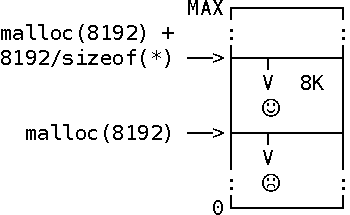
\includegraphics[width=\marginparwidth]{thumbnails/segfault}
  %   \captionof{figure}{\label{fig:segfault}Segmentation fault!}}
  如图\ref{fig:segfault}所示,
  虽然系统为你开辟出了8k的内存,但\texttt{malloc(3)}返回的指针指向这段内存的起始位置,也就
  是8k下面的那条线。而你如果想把这段内存当栈用的话,应该把指针挪上去。为啥?因为栈是向下长的啊。如果
  不挪下去,直接向下长,就长到别人的地址空间里去了,这就是segmentation fault。所以要像下面
  这样,把指针挪上去:
\begin{ccode}
child_stack = (void **) malloc(8192) + 8192/sizeof(*child_stack);
\end{ccode}  
\end{enumerate}


\section{构建和谐社会}
\label{sec:ipc}

Interprocess synchronization,很多书都把它翻译成“进程间同步”。看到“同步”二字,你脑子里闪现出来的
是啥?十之八九是“齐刷刷、齐步走”吧。所以说,这样的翻译是典型的望文生义,害
人。Synchronization这个词,在不同的场合,可以有不同的理解,比如说,俩人相互校对一下手表,把
时间调一样了,这就叫synchronization。再比如,Unix命令行都提供一个不那么常用的命
令\texttt{sync},显然就是 synchronization 的缩写,干什么使呢?举例而言,假设你要把一个大文
件(比如电影)从硬盘拷贝到U盘上,
\begin{shcode}
  cp Forrest.Gump-1994.mp4 /mnt
\end{shcode}
敲完这条命令,你一回车,会发现命令马上就结束了。难道说这么快就拷贝完了?那可是一
个8G大的4K高清电影,怎么可能嘛。的确,没拷贝完,但由于拷贝大文件要花费很长的时间,也许要一
个多小时,而且这件事情的优先级不那么高,所以,Unix怕你等得不耐烦,就先把命令行提示符
(\texttt{\$})返还给你,于是你就可以该干吗干吗了。系统会在后台慢慢去完成拷贝工作。那如果我
非要“立等可取”呢?那你就敲\texttt{sync},这时候你会发现,命令行提示符(\texttt{\$})老半天
也出不来,直到硬盘和U盘上的两个电影文件“sync”(一致)了,提示符才出来,也就是拷贝结束了。

上面两个例子里,synchronization的意思都差不多,是“让它们变得一
致”的意思,有点“齐步走”的感觉。而进程间的synchronization就不是这样了,它强调的是“和谐共处,
不要打架”。前面说过,系统里进程多,资源少,也就类似于饭桌上筷子多,肉少,synchronization就
是要想办法避免多双筷子叉到一块肉上的尴尬。

\subsection{工具箱和瑞士军刀}
\label{sec:toolbox}

\mpic{pg_0099}现在看看幻灯片第98页,Interprocess communication,进程间通信。
很显然,synchronization要解决的是进程间关系的问题,如果系统是单进程(单任务)的,就没啥好和
谐的了。先看看幻灯片上的例子:
\begin{shellcode}
  unicode skull | head -1 | cut -f1 -d' ' | sm -
\end{shellcode}
\marginpar{{\tikz \node[scale=10]{\dejavu ☠};}}面对这么长一条命令,别慌,别不耐烦,学计科、
学编程的人,总该有个有条有理的思维、做事习惯才行。怎么算是有条有理?大事化小,一步步尝试。
\begin{enumerate}
\item 既然看不太懂,先拷贝到命令行上运行一下呗。运气好的话,你会看到一个巨大的骷髅头出现在
  屏幕上。什么情况?
\item 试试:
  \begin{shellcode}
    unicode skull | head -1 | cut -f1 -d' '
  \end{shellcode}
  输出结果是个小骷髅头({\dejavu ☠})。
\item 再试试:
  \begin{shellcode}
    unicode skull | head -1
  \end{shellcode}
  输出是“\verb|☠ U+2620 SKULL AND CROSSBONES|”。
\item 再试试:
  \begin{shellcode}
    unicode skull
  \end{shellcode}
  输出是:
\begin{verbatim}
☠ U+2620 SKULL AND CROSSBONES
💀 U+1F480 SKULL
🕱 U+1F571 BLACK SKULL AND CROSSBONES
\end{verbatim}
\end{enumerate}
还有啥不明白吗?现在这命令里就俩单词了,\texttt{unicode}和\texttt{skull},不认识的话可以
查字典。
\begin{enumerate}
\item 不知道\texttt{unicode}是干吗的,你可以\texttt{man unicode};
\item 然后,\texttt{man head},就知道它是要取前一条命令输出的第一行;
\item 然后,\texttt{man cut},就知道这是要把这行最开头的东西cut出来;
\item 然后,\texttt{man sm},就知道为啥能看到大骷髅了。
\end{enumerate}

如果你遭遇了“\texttt{Command not found}”,那就
\begin{shellcode}
  sudo apt install unicode sm
\end{shellcode}
现在就剩下一个问题了,命令中的竖杠(\texttt{|})是干啥用的?其实你已经能猜出个大概齐了,用
它可以把几个命令串起来。没错,这竖杠叫pipe,“管子、管道”的意思。

Unix系统有一个很著名的设计原则,do one thing and do it well,做一件事,并把它做好。基于这一
原则,Unix系统为用户提供了无数的小命令,每个小命令只做一件事,并且做的非常好。比如说我们最
常用的\texttt{ls}命令吧,说起来无非就是要列出目录中的内容呗。但是,你可以
\begin{multicols}{2}
  \begin{itemize}
  \item[-l] 列出详细信息;
  \item[-t] 按时间排序;
  \item[-S] 按大小排序;
  \item[-r] 倒着排序;
  \item[-R] 列出子目录里的内容;
  \item \texttt{man ls} for more
  \end{itemize}
\end{multicols}
\mfig{pg_0354}{Do one thing and do it well.}
% \marginpar{%
%   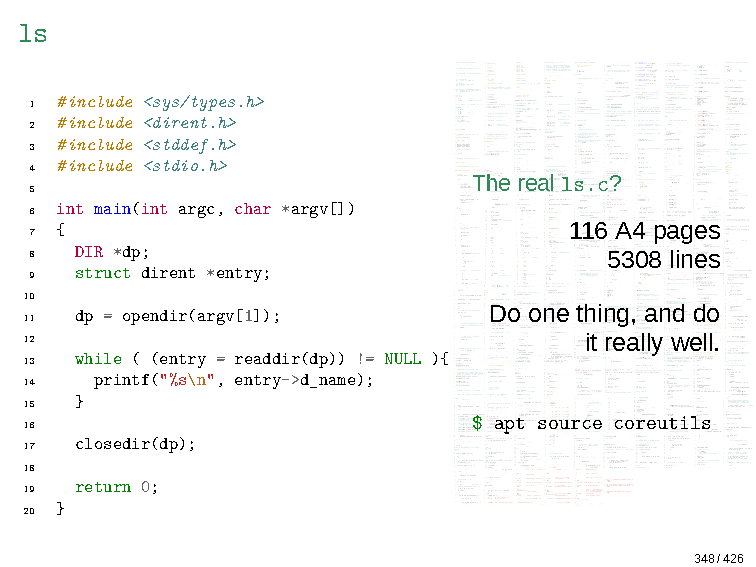
\includegraphics[width=\marginparwidth]{thumbnails/pg_0354}
%   \captionof{figure}{\label{fig:pg_0354}Do one thing and do it well.}}%
除了提供数不清的选项,还要提供一个详尽的手册供用户查阅。这就叫do it
well。图\ref{fig:pg_0354}里左边那个\texttt{ls.c}是我写的,右边的是我们系统里
的\texttt{ls.c}。这个对比能帮我们清醒认识一下什么是do it well,它绝不仅仅是技术,更是态度,
是耐心。

软件世界里,还有另一个很流行的设计模式,瑞士军刀模式。也就是开发一个工具,让它能做很多事情。
这一思想的范例就是IDE,Integrated Development Environment,集成开发环境,比如MS Visual
Studio, Eclipse,等等。那么,是工具箱好,还是瑞士军刀好?我觉得要看应用场景。比如说吧,如果
你在家修理自行车,是用工具箱里的扳手、钳子、改锥,还是用钥匙串上的瑞士军刀啊?如果你骑车出
去旅行,你是驮一个大工具箱,还是带一把像样的瑞士军刀呢?

虽说是各有各的应用场合,我个人还是很偏爱工具箱。仔细想想看,IDE无非包括如下一些功能模块:一
个编辑器,一个编译器,一个调试器,外带其它一些辅助功能,比如用鼠标拖控件。那么,最好的IDE肯
定就是:
$$\text{最好的编辑器} + \text{最好的编译器} + \text{最好的调试器}$$

\begin{itemize}
\item 世上最强大的编辑器是Emacs,这一点没人能否认。Emacs的设计目标就是,你装了
  个Unix或者Linux系统,不需要装任何其它软件,只要装一个Emacs就够了,它能帮助你完成所有的任
  务。也就是说,除了编程,你还可以用它写论文、做幻灯片、浏览网页、收发邮件、聊天、听歌、看
  照片、玩游戏……目前,好像除了直接在Emacs里看电影还不行,其它的都实现了。

  Emacs如此「大一统」的设计目标显然有违do one thing, and do it well的设计原则啊。但好
  在Emacs是模块化的,它的每一个功能模块都绝对遵循do one thing, and do it well原则。你不喜欢
  那些功能,可以不装它。换言之,Emacs就是个大工具箱;
\item 世上最强大的编译器是GCC,GNU Compiler Collection,其中包括了\texttt{gcc, g++,
    gcj}……等若干编译器。Linux内核的数千万行代码就是用\texttt{gcc}编译的;
\item 世上最牛的调试器是\texttt{gdb},有好几本书专门来介绍它的强大功能。
\end{itemize}

没有任何一个IDE把上述三样最优秀的工具集成到一起。如果说有,那就是Emacs。Emacs虽然只是编辑器,
但它可以很方便地调用\texttt{gcc}和\texttt{gdb}。也许你会说「Emacs不能拖控件啊」,没错,但在
我看,拖控件并不总是一个受人欢迎的功能,至少在系统编程的时候,它毫无用处。而且,从学习的角
度来说,拖控件,用鼠标编程,绝对是一个非常恶劣的习惯,因为这根本就是在逃避学习。“鼠标化的IDE”隐
藏了很多学生应该了解的技术细节。我们的绝大多数同学居然不知道C程序是要编译之后才能运行的,
他们以为写好了程序,只要「按那个“感叹号”按钮」就可以了。这就是“鼠标教学”的成果(你肯定知
道C编程这门课不归我管)。Emacs可以帮助你克服“鼠标依赖”,强迫你熟练地使用键盘。

好了,越扯越远了,扯回来,Unix给了我们一个大工具箱,同时也给我们提供了把小工具组合成大工具
的若干机制,pipe\texttt{(|)}就是其中之一。通过pipe,前一个命令的输出可以被传递给后一个命令,
如此串下去,可以形成一条规模可观的“流水线”,进来的是钢铁,出去的就是汽车了。

再来看幻灯片第98页,进程间通信必须要解决三个问题:
\begin{enumerate}
\item 一个进程怎样给另一个进程传递信息。现在,我们至少会用pipe了;
\item 不要打架,和谐共处;
\item 顺序问题。以流水线为例,你必须要等汽车轱辘过来了,才能实施拧螺丝的操作。以幻灯片上的
  长命令为例,后面的命令一定要等前面的命令完成之后,才能动作。
\end{enumerate}

\subsection{IPC的两种方式}
\label{sec:ipc-1}

IPC有两个基本方式,一是共享内存;二是信息传递。很显然,共享内存只可能发生在同一台电脑里的若
干进程之间。换言之,在不同电脑上的进程,如果要相互通信的话,只能通过第二种方式,message
passing,也就是网络传输方式。网络传输也可以(而且经常)用在同一台电脑上的进程之间。现在学个
网络命令:
\begin{shellcode}
  ip a 
  ip --color=auto a #豪华版
\end{shellcode}
用这条命令可以列出你电脑上所有网卡的信息。不出意外的话,你看到的第一块网卡应该
叫“\texttt{lo}”,loopback的缩写,“回环”的意思。这个\texttt{lo}是个虚拟网卡,专门就是用于本
机上的进程间通信。举个例子,Unix平台的图形界面,也就是传说中的Xwindow,就是通过网络传输实现
的。比如说,你要用\texttt{xpdf}打开一个PDF文件。\mfig{xwin1-ascii}{How Xwindow works}
% \marginpar{%
%   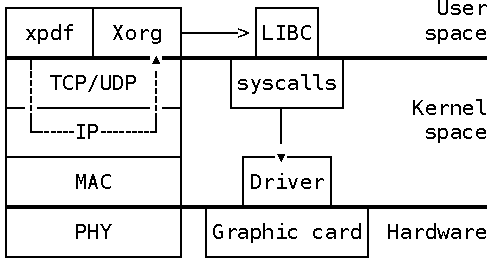
\includegraphics[width=\marginparwidth]{thumbnails/xwin1-ascii}
%   \captionof{figure}{\label{fig:xwin1-ascii}How Xwindow works}}%
如图\ref{fig:xwin1-ascii}所示,\texttt{xpdf}(图形界面客户端)会把“打开一个窗口”的请求,通
过TCP/IP协议栈,发送给\texttt{Xorg}(图形界面服务器)。然后再
由\texttt{Xorg}通过LIBC调用syscall,向操作系统发出请求,操作系统再通过调用显卡驱动程序,驱
动显卡,最终把图形窗口显示在屏幕上。

图\ref{fig:xwin1-ascii}中,我们需要注意一下TCP/IP协议栈在计算机系统中的位置。协议栈,除了物理层之
外,都是软件实现的。协议栈的应用层在User space;传输层、网络层、链路层在Kernel space;物理
层,也就是网卡,当然是属于硬件范畴。\texttt{xpdf}和\texttt{Xorg}都处于协议栈的应用层,它们
之间的通信,是在协议栈里绕了一圈(应用层{\dejavu ➜}传输层{\dejavu ➜}网络层{\dejavu ➜}传输
层{\dejavu ➜}应用层)才完成的。而且,由于客户端(\texttt{xpdf})和服务器(Xorg)在同一台电
脑上,所以这一圈没有绕到物理层去,到IP层就通过虚拟网卡(\texttt{lo})绕回来了。%

\mfig{xwin2-ascii}{How Windows works}
% \marginpar{%
%   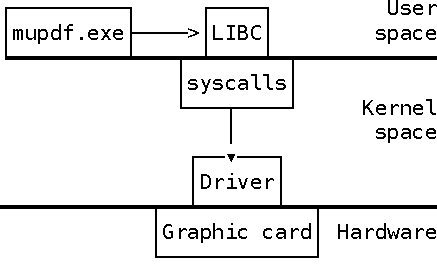
\includegraphics[width=\marginparwidth]{thumbnails/xwin2-ascii}
%   \captionof{figure}{\label{fig:xwin2-ascii}How Windows works}}%
现在,问题来了,干吗这么绕来绕去,像Windows那样(图\ref{fig:xwin2-ascii})直截了当不好吗?这又要
讲讲历史了。Unix天生是个多用户系统,而多用户之间有通信需求啊,所以,Unix很早就有了对联网的
支持,而图形界面的出现则要晚一些。于是,在搞图形界面开发的时候,面对
图\ref{fig:xwin1-ascii}和图\ref{fig:xwin2-ascii}所示的两种方案,选择的时候就要纠结一下了。直截了当(
图\ref{fig:xwin2-ascii})的好处是快,但远程桌面怎么办?那就不得不再来一套网络方案(
图\ref{fig:xwin1-ascii})。而实际上,网络方案可以同时满足本机和远程这两种进程间通信的需求,那何必
再多此一举地搞一套“直截了当”方案呢?于是,Unix就天生支持远程桌面了。
\mfig{xwin3-ascii}{X for remote}
% \marginpar{%
%   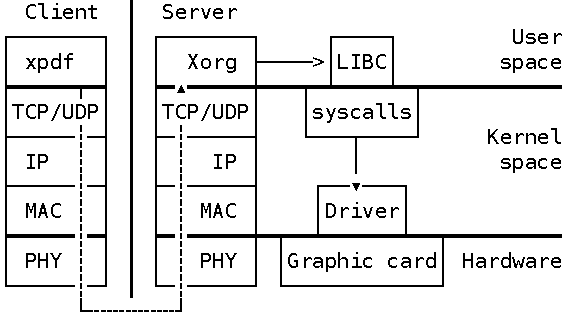
\includegraphics[width=\marginparwidth]{thumbnails/xwin3-ascii}
%   \captionof{figure}{\label{fig:xwin3-ascii}X for remote}}%
具体而言,如果客户端和服务器不在同一台电脑上的话(图\ref{fig:xwin3-ascii}),和
图\ref{fig:xwin1-ascii}很类似,客户端(\texttt{xpdf})的服务请求经过
\begin{center}
  应用层{\dejavu ➜}传输层{\dejavu ➜}网络层{\dejavu ➜}链路层{\dejavu ➜}物理层
\end{center}
到达网卡,然后顺着网线到达服务器电脑,进入网卡之后,经过:
\begin{center}
  物理层{\dejavu ➜}链路层{\dejavu ➜}网络层{\dejavu ➜}传输层{\dejavu ➜}应用层
\end{center}
到达\texttt{Xorg}。之后发生的事情就和图\ref{fig:xwin1-ascii}中右半部分的情形一模一样了。

而MS Windows起源于MS-DOS,天生是个单用户系统。当初,1980年,DOS是比尔·盖茨花五万美金,从一
个西雅图码农手里买来的。买来之后再加班加点,改头换面,为了赶工期,根本就没开发网络功能。后
来,比尔·盖茨靠DOS发了财之后,把苹果的图形界面“借鉴”了过来,就有了Windows,但还是没有联网功
能。所以,Windows是先有图形界面,后有网络支持的。所以,它肯定是先有“直截了当”方案,然后再补
充一个远程桌面出来。客观来讲,“直截了当”的好处还是显而易见的,所以,在Xwindow雄霸Unix几十年
之后,要逐渐被新一代图形界面机制(Wayland)取代了。

\subsection{生产者与消费者}

楼下保安说,计算机里就俩进程,一个是生产者(producer),另一个是消费者
(consumer)。\mpic{pg_0100}就像幻灯片第99页上画的那样,一个进程把要打印的文件生产出来,放
进缓存区(buffer),打印机守护程序(daemon)把它取走,打印掉。编译器编译出汇编代码,放
进buffer里,汇编器把它取走吃掉,然后拉出二进制的目标文件,放进buffer里,再被倒霉的链接器
(loader)取走,皱着眉头、捏着鼻子、含着眼泪吃掉。上述例子中的生产者和消费者是通过共享内存
(buffer)来进行通信的。很显然,要想让通信保持和谐(synchronization)的话,必
须:\mpic{pg_0102}
\begin{itemize}
\item Buffer里没东西的时候,不许消费;
\item Buffer满了的时候,不能生产。
\end{itemize}
把这两句话用程序表达出来,就是幻灯片第101页上的那样,这两段小程序显然是用C语言写的伪代码
(pseudocode),左边那段是生产者,右边的是消费者。那怎么来定
义“满了”和“空了”呢?人是很聪明的,眼睛一看就知道是“满了”还是“空了”。但机器不
行,你得给它编程序。看看幻灯片第102页上的那张画,那就是个典型的buffer,一个环形数组,里面
有8个位置可以放东西。这buffer上画了两个指针:
\begin{description}
\item[in] 指向下一个空位置。也就是说,生产者生产出来的东西都是放到in所指的位置里,然后in
  再顺时针前移一个位置;
\item[out] 指向第一个满位置。也就是说,消费者饿了的话,就从out所指位置拿东西去消费,然后
  out再顺时针前移一个位置。
\end{description}
\mpic{pg_0103}
我们可以借助in、out这两个指针来定义“满了”和“空了”。假设消费者睡着了,而生产者在不断生产,那
么in指针就会不断顺时针前移,当它和out重合的时候,\(in == out\),buffer就满了,
对吧?那么,我们再反过来假设生产者睡着了,而消费者在不断地吃。类似地,当两个指针重合
的时候,肯定是buffer空了。问题来了,如果我们用“\(in == out\)”来定义“满了”,那么就必须另想个
办法来定义“空了”,对吧?答案在幻灯片第103页上。\mpic{pg_0104}
\begin{itemize}
\item 用“\(in == out\)”来定义“空了”;
\item 用“\((in+1)\%BUFFER\_SIZE==out\)”来定义“满了”。其实,就是用
  “\((in+1)==out\)”来定义“满了”。只不过如果不对\(BUFFER\_SIZE\)取模
  (\(\%\))的话,“\(in+1\)”是会加到天上去的。取模就是为了把“\(in+1\)”限制
  在\(BUFFER\_SIZE\)以内。
\end{itemize}
这样定义的话,“满了”和“空了”显然不会再发生冲突了,唯一的小毛病就是,要浪费掉buffer中的一个
位置,因为它不可能有真正满的时候了。

解决了“满了”与“空了”的定义问题,幻灯片第102页上的小程序就升级为第103-104页上
的样子了。程序开始的时候,in和out都是0,表示buffer是空的。然后,生产者生产,消费者消费。如
果buffer满了,生产者就等待(死循环);如果buffer空了,消费者就等待(也是死循环)。
\mpic{pg_0105}

\subsection{Pipe}
\label{sec:pipe}

Pipe是进程间通信的常用工具。幻灯片第105页是以“\texttt{ls | wc -l}”这个小命令为例,来说明它
的实现机制\citetitle[Sec.~44.1]{kerrisk:2010:lpi:1869911}。很显然,\texttt{ls}在这里是生产
者,\texttt{wc}是消费者,它们两位通过一根大管子来传递信息。注意三点:
\begin{enumerate}
\item Pipe里的信息传输是单向的;
\item Pipe里传输的是字节流(byte stream)。Byte stream这个概念在Unix里很重要。
  第\ref{sec:write}节中我们提到过,in Unix, everything is a file。现在可以再补充一
  句,every file is a byte stream。这一设计思想大大简化了操作系统的设计。很显然,做为操作系
  统,Unix没什么理由去关心文件的内容,那么自然也就无需去判断文件的类型、大小之类的细节,因
  此也就省去了许多琐碎的工作。无论来了什么文件,只要找一条管子,让它从这头流进去,管子的另
  一头要么是个进程,要么是个文件,流过去就完事了。接收端如果是个进程,它自己负责解读
  (interpret)收到的数据。比如说,有个PDF文件吧,
  \begin{itemize}
  \item \texttt{xpdf}的解读方式是,打开一个窗口,把它漂亮地显示出来;
  \item 如果是\texttt{cat}收到了它,你试试\texttt{cat talk.pdf},看到的会是一堆乱码;
  \item 如果是用\texttt{hexdump}解读它呢,你试试\texttt{hd talk.pdf};
  \end{itemize}
  \mpic{pg_0106}总之,解读文件的内容,是应用层软件的工作,操作系统不操心。至于说用什么工具
  去解读,那是你的自由,操作系统也不操心。
\item 在“\texttt{ls | wc -l}”这个例子中,\texttt{ls}向pipe里写,\texttt{wc}从pipe里读。如果
  这边什么也没写进去,那边自然就什么也读不到,在这种情况下,“读者”就要等着(blocked,阻断)。其
  实,这就是我们前面说的,buffer如果是空的,消费者就不能消费。
\end{enumerate}

简单介绍一下幻灯片第105页上出现的STDIN (fd 0), STDOUT (fd 1)。前面在第\ref{sec:write}节中
讲\texttt{write(2)}的时候我们说过,任何一个进程都至少要打开三个文件:STDIN, STDOUT, STDERR。
而且,一个进程打开的所有文件都被记录在一张表里,这张表叫File descriptor table (FDT)。举个例
子,假如我们现在写个helloworld小程序:
\begin{shellcode}
  vim hello.c
\end{shellcode}
很显然,敲完上面的命令,一回车,系统里就多了个进程,该进程的FDT大致如图\ref{fig:fdt}所
示\mfig[.3]{fdt}{File descriptor table}。注意,这张表的索引,前三个是固定不变的:
\begin{itemize}
\item[0] - STDIN,标准输入;
\item[1] - STDOUT,标准输出;
\item[2] - STDERR,标准错误。
\end{itemize}

现在,顺带学两个小命令:
\begin{enumerate}
\item \texttt{pidof vim},很显然,这是要得到\texttt{vim}的进程号。想了解更多,显然你该
  \texttt{man pidof};
\item \texttt{lsof -p \$(pidof vim)}。这命令看着有点高级,假如你闷头敲进去,执行一下,输出
  结果就是\texttt{vim}进程打开的所有文件。\texttt{\$(cmd)}是要分两步完成一个任务:
  \begin{enumerate}
  \item 执行\texttt{cmd}命令。在我们的例子里,要执行的命令就是\texttt{pidof vim};
  \item 用\texttt{cmd}命令的输出结果,替换掉\texttt{\$(cmd)}这个字符串。在我们的例
    子里,自然就是用\texttt{pidof vim}的输出结果(也就是一个进程号)来替换。替换之后,
    \begin{center}
      \fbox{\texttt{lsof -p \$(pidof vim)}} $\Rightarrow{}$ \fbox{\texttt{lsof -p 888}}
    \end{center}
    其输出结果自然就是第888号进程打开的所有文件(假设进程号是888的话),也就是FDT表中的内
    容。
  \end{enumerate}
\end{enumerate}

Unix命令的运行结果通常都是输出到屏幕上,也就是STDOUT,标准输出。但有的时候我们不想这样,于
是你可以“输出重定向”(output redirection)。比如,
\begin{itemize}
\item \texttt{ls > ls.out},就是把\texttt{ls}的运行结果输出到文件\texttt{ls.out};
\item \texttt{ls | wc -l},就是把\texttt{ls}的运行结果输出到pipe,也就是幻灯片上画的那样。
\end{itemize}

幻灯片第105页的下半部分,是顺带介绍个挺有用的小命令\texttt{tee}。这命令显然就读做“T”,而字
母“T”,从外形上看,分叉了。命令\texttt{tee}就是要分叉输出到两个方向,一是标准输出;二是文件。

\mpic{pg_0107}幻灯片第106页上画出了pipe的工作原理,这根大管子实际上就是内核里的一个buffer,
生产者把东西丢进去,消费者把它拿出来而已。“丢进去”调用的肯定是\texttt{write(2)},“拿出来”
调用的肯定是\texttt{read(2)}。很简单吧。幻灯片最下面的命令,不用解释了吧。如果你嫌buffer不够大,
也可以修改这个文件。

\subsubsection{\texttt{pipe(2)}}
\label{sec:pipe2}

前面我们介绍的是pipe的工作原理,现在来看看怎么用\texttt{pipe(2)} syscall来编程\citetitle[Sec.~44.2]{kerrisk:2010:lpi:1869911}。
\mpic{pg_0108}幻灯片第107页上,首先给出的就是它的prototype,函数原型。
\begin{ccode}
#include <unistd.h>

int pipe(int fd[2]);
\end{ccode}
看着非常简单,用着也很简单。但在调用\texttt{pipe(2)}之前,你要先准备好\texttt{fd[2]}这个数
组,实际上也就是告诉\texttt{pipe(2)},创建出来的大管子,两头该分别插在哪儿。
\texttt{pipe(2)}会把“读端”插在\texttt{fd[0]}上;把“写端”插在\texttt{fd[1]}上。换句话说,调
用完\texttt{pipe(2)}之后,你就可以\texttt{write(fd[1])}、\texttt{read(fd[0])}了。

Pipe是用来做进程间通信的,所以显然要有两个进程参与。\mfig[.4]{pipe1}{自己和自己玩}如果像
图\ref{fig:pipe1}那样,自己读、自己写,不是不可以,实在是没啥意义。所以,\texttt{pipe(2)}
通常都是和\texttt{fork(2)}配合使用的,就像幻灯片的下半部分画的那样。你可以这样来理解a、b这
两张图:
\begin{itemize}
\item[a)] 一个进程先调用了\texttt{pipe(2)}造了一个大管子,然后就自己和自己玩。玩腻了之后,
  他调用\texttt{fork(2)}生了个儿子,陪他一起玩。由于子进程复制了父进程的一切,自然也复制了
  这个大管子。这就是图a呈现给我们的样子。
\item[b)] 两个进程,一个读,另一个写。读的这个,显然它不写,所以用不到写的那端,于是它把自
  己的“写端”(\texttt{fd[1]})关闭了。同理,另一个进程关闭了自己的“读端”(\texttt{fd[0]})。
  这就是图b给出的样子。「不用就非要关闭吗?」没错,不需要的那端必须关闭,否则会有问题。是这
  样,Pipe在用完之后,显然是应该释放掉的吧,毕竟它是要耗资源的嘛。那么问题来了,怎么才知
  道“用完”了呢?比如说“读端”吧,当“写端”写完了,它也就读完了,对吧。但它怎么知道“写端”写完
  了呢?\texttt{pipe(7)}手册上说,当和“写端”相连的所有\texttt{fd[]}都关闭了之后,如果“读端”继
  续读,那么它读到的会是EOF(End Of File),也就是\texttt{read(2)}的返回值为0,于是它就知道
  读完了。所以,如果我们不关闭没用的那端,“读端”就永远读不到EOF,它会一直以为“写端”还没写完,
  于是就一直等着(blocked),pipe也就永远不会被释放掉。
\end{itemize}

\mpic{pg_0109}幻灯片第108页上是个简单的\texttt{pipe(2) + fork(2)}的例子,其中用到的
\texttt{read(2), write(2)}这些syscall前面(第\ref{sec:syscall}节)都见过了。自己试试吧。
\begin{itemize}
\item 下载:\url{https://cs6.swfu.edu.cn/~wx672/lecture_notes/os/src/proc/simple_pipe.c}
\end{itemize}

\subsubsection{Named Pipe (FIFO)}
\label{sec:fifo}

In Unix, everything is a file。这句话我们提过很多次了,既然什么东西都可以是文件,那么在内存
里开辟出来,用于进程间通信的buffer当然也可以是文件了。没错,所谓named pipe,有名字的管子,
也叫FIFO,本质上就是这样一个带名字的buffer。为啥要给buffer起名字呢?因为,上一节中讲的普通
没名字pipe并不能满足所有的需求。没名字的pipe只能在父、子进程间使用。如果是素不相识的两个进
程,无名pipe就不好使了。因为,一个进程创建了pipe,别人都不知道它的存在,当然就找不到它,当
然也就没法用它。子进程之所以能找到它,是因为\texttt{fork(2)}之后,子进程天然就继承了老爸
的pipe,所以爷俩共用一个管子就顺理成章了。

\mpic{pg_0110}我们来看看幻灯片第109页上的小例子。
\begin{enumerate}
\item \texttt{mkfifo myfifo},这是要在当前目录里创建一个新管子,名字叫\texttt{myfifo}。之后,
  用\texttt{ls -lF myfifo}看一眼的话,输出结果大致是下面这个样子:
\begin{verbatim}
prw-r--r-- 1 wx672 wx672 0 Apr 17 14:45 myfifo|
\end{verbatim}
  注意打头和结尾的两个字母:
  \begin{itemize}
  \item[\texttt{p}] 代表pipe;
  \item[\texttt{|}] 也是代表pipe。因为\texttt{ls}的时候加了选项“\texttt{-F}”,所以文件名的结
    尾处会标出文件类型。
  \end{itemize}
\item \texttt{echo hello > myfifo},这是要把\texttt{hello}这个字符串写到管子里去;
\item \texttt{cat myfifo},这是要从管子里读取数据;
\item \texttt{echo hello | tee myfifo},这是先把\texttt{hello}写进无名pipe里去。在pipe的另
  一头,用\texttt{tee}分叉输出,既输出到屏幕,还输出给\texttt{myfifo};
\item \texttt{wc myfifo},用\texttt{wc}处理\texttt{myfifo}里的东西,也就是计算字数。
\end{enumerate}

再看看幻灯片第110页上的小程序,它的完整版
在\citetitle[Sec.~13.6, p544]{matthew2008beginning}。

\end{document}

%%% Local Variables:
%%% mode: latex
%%% TeX-master: t
%%% End:
